\documentclass[																					%IRAS Vorlage
  a4paper,
  oneside,
  nexus,
  11pt,																									% <10pt, 9pt>
																												%style=screen,
																												%sender=bottom,
  blue,																									% <orange, green, violet>
																												%rgb, <cmyk>
																												%mono,
																												%extramargin,
																												%marginleft, <marginright>
  ]{tubsreprt}

\usepackage[utf8x]{inputenc}
\usepackage[ngerman]{babel}
\usepackage[square]{natbib}
\usepackage{graphicx}
\usepackage{amsmath}                   									 % Packages für Formeln
\usepackage{amsthm}																			 % -||-
\usepackage{amsfonts}																		 % -||-
\usepackage{amssymb}																		 % -||-
\usepackage{lscape}																			 % Querformatiges Beschreiben einzelner Abschnitte 
																												 %mit \begin{landscape} Text \end{landscape}
																												

\usepackage{tikz} 																			 % TikZ - ein geniales Zeichentool vor allem für Skizzen oder Schemata, Programmabläufe, etc.
\usepackage{bibgerm}																		%bibliography deutsch
																										 
\usepackage{pgf}																				 % Für Tikz
\usepackage{pgfplots} 																	 % Plots mit TikZ
\usetikzlibrary{shapes,backgrounds, arrows, positioning, trees, shadows}% Bibliotheken für Tikz
\usepackage{pgfgantt}																		 % Zum Erstellen eines Gantt-Charts

\graphicspath{{./graphics/}}														 %greift auf den Unterordner "graphics" zu
\usepackage{pdfpages}																		 %ermöglicht das Einbinden von PDF-Datein

%===============================================================
%
%	Hyperlinks im Dokument
%
%---------------------------------------

\usepackage[
	pdftex,
  hidelinks,%
  linktocpage, breaklinks
]{hyperref}																							% Package für Lesezeichen und Verlinkungen

%===============================================================
%
%	Glossary
%
%---------------------------------------
\usepackage[nonumberlist,acronym,section]{glossaries}

 
																												%nonumberlist: no page numbering
																												%acronym: abbreviations list
																												%toc: entry in table of contents
																												%section: in toc placed at section level
																												%nopostdot: no dots after description
				
\newglossary[slg1]{symbolslist}{syi}{syg}{List of Symbols}																			% symbols
\newglossary[alg]{acronymlist}{acr}{acn}{List of Abbreviations}																	% abbreviations	

\makeglossaries

\AtEndDocument{\glsaddall}																%füge alle Symbole dem Verzeichnis zu

%-----------------------------------------------------------------


																													%Makros für eine erleichterte Eingabe wiederkehrender Befehle:
\newcommand{\abb}[1]{Abbildung~\ref{#1}}
\newcommand{\tab}[1]{Tabelle~\ref{#1}}
\newcommand{\glg}[1]{Gleichung~\ref{#1}}
\newcommand{\kap}[1]{Kapitel~\ref{#1}}
\newcommand{\abschn}[1]{Abschnitt~\ref{#1}}
\newcommand{\anh}[1]{Anhang~\ref{#1}}

\newcommand{\ul}{\underline}
\newcommand{\ol}{\overline}
\newcommand{\tb}{\textbf}
\newcommand{\ts}{\textsl}

\newcommand{\kalman}{\textsc{Kalman}-Filter }

%===============================================================
%
% Farben
%
%-------------------------------

\definecolor{ilr-blue}{RGB}{44,79,162}
\definecolor{light-blue}{RGB}{220,220,255}
\definecolor{gray90}{gray}{0.9}
\definecolor{gray80}{gray}{0.8}
\definecolor{gray60}{gray}{0.6}
\definecolor{gray50}{gray}{0.5}
\definecolor{gray40}{gray}{0.4}
\definecolor{gray20}{gray}{0.2}

%===============================================================
%
% Titelseiten
%
%-------------------------------

\title{\LARGE Projektarbeit SS 2019 \newline Analyse einer CubeSat-basierten ADR-Mission}
\subtitle{Institut f\"ur Raumfahrtsysteme}
\author{\small Florian Czorny, Frederik Sch\"afer, Marc Strempel, Oussama Mouhaya, Valentina Dietrich}

%---------------------------------------------------------------
% Titelbilder + IRAS Logo (Deckblatt)
%---------------------------------------------------------------

\logo{\includegraphics{iras_logo.jpg}} 
\titlepicture{doctor_pop2009.jpg}

%===============================================================
% Hurenkind bzw. ein Schusterjunge 
%---------------------------------------------------------------
\clubpenalty         = 10000
\widowpenalty        = 10000
\displaywidowpenalty = 10000
%===============================================================
% Hauptfunktion
%---------------------------------------------------------------

\begin{document}																												%Erstellung des Schreibdokumentes 

  \maketitle[image] 																										%[<plain/image/imagetext>,<logo=left/right>]

 \includepdf[pages=-]{./header_first/Aufgabenstellung_PA_SS19.pdf}			%PDF-Datei wird hinzugefügt 
 \chapter*{Eidesstattliche Erkl\"arung}

Wir erklären hiermit an Eides Statt, dass wie die nachfolgende Arbeit selbständig und nur unter Zuhilfenahme der angegebenen Literatur angefertigt haben.


\vspace{2cm}
\tikz\draw (0,0) -- (7,0);

Datum, Unterschrift Florian Czorny
  
\vspace{2cm}
\tikz\draw (0,0) -- (7,0);

Datum, Unterschrift Frederik Schäfer
  
\vspace{2cm}
\tikz\draw (0,0) -- (7,0);

Datum, Unterschrift Marc Strempel

\vspace{2cm}
\tikz\draw (0,0) -- (7,0);

Datum, Unterschrift Oussama Mouhaya
 
\vspace{2cm}
\tikz\draw (0,0) -- (7,0);

Datum, Unterschrift Valentina Dietrich

 \tableofcontents																												%Erstellung eines Inhaltsverzeichnisses
  \newpage
	%\newglossarystyle{rhg-altlong4col}{\glossarystyle{altlong4col}
		\glossarystyle{altlong4col}
			\setlength{\glsdescwidth}{0.7\textwidth}
	
	\include{./header_verzeichnisse/symbolverzeichnis1}					
	
\newacronym{ADC}{ADC}{Attitude Determination and Control}
\newacronym{ADR}{ADR}{Active Debris Removal}
\newacronym{COTS}{COTS}{Comercially of the Shelf}
\newacronym{COTS}{COTS}{Center of Mass}
\newacronym{ECSS}{ECSS}{European Cooperation for Space Standardization}
\newacronym{EPS}{EPS}{Electrical Power System}
\newacronym{GMAT}{GMAT}{General Mission Analysis Tool}
\newacronym{GNC}{GNC}{Guidance, Navigation and Control}
\newacronym{GPS}{GPS}{Global Positioning System}
\newacronym{GUI}{GUI}{Graphical User Interface}
\newacronym{LEO}{LEO}{Low Earth Orbit}
\newacronym{MarCO}{MarCO}{Mars Cube One}
\newacronym{NEA}{NEA}{Near Earth Asteroid}
\newacronym{NEO}{NEO}{Near Earth Object}
\newacronym{PDMS}{PDMS}{Polydimethylsiloxan}
\newacronym{PMAD}{PMAD}{Power Management and Distribution}
\newacronym{QuSAD}{QuSAD}{SQL-Based CubeSat Analysis and Design Tool}
\newacronym{RCS}{RCS}{Reaction Control System}
\newacronym{ROE}{ROE}{Relative Orbital Elements}
\newacronym{RvD}{RvD}{Rendezvous and Docking}
\newacronym{TRL}{TRL}{Technology Readiness Level}
	
	\chapter{Einleitung}
		\section{Motivation}

\begin{flushleft}
		Der Weltraum ist vermutlich unendlich, jedoch nicht der Platz in den Erdumlaufbahnen. Seitdem ersten Satelliten Sputnik 1, welcher am 04. Oktober 1957 in die Erdumlaufbahn geschossen wurde, kommen immer mehr Satelliten hinzu. Diese bilden die Grundlage unserer modernen Kommunikation und sind aus dem menschlichen Alltag nicht wegzudenken.
Neben den bereits vorhandenen Satelliten werden jedes Jahr neue in den Erdorbit befördert. Beim Start von Satelliten und Sonden bleiben Raketenstufen in der Erdumlaufbahn zurück, welche aufgrund ihrer Manövrierunfähigkeit eine Gefahr für Menschen und Maschinen im Weltall bilden. Moderne Low-Earth-Orbit (LEO)-Satelliten werden so entwickelt, dass diese am Ende ihrer Lebensspanne wieder in die Erdatmosphäre eintreten und verglühen. 
Sollten diese Objekte eine Funktionsstörung haben oder beschädigt sein, können diese den selbst initiiert Wiedereintritt nicht durchführen. Da diese Objekte unkontrolliert im Weltraum treiben, besteht die Möglichkeit einer Kollision mit anderen Satelliten. Dabei zersplittern die Trümmer in einem Kaskadeneffekt und weitere Kollisionen sind unumgänglich. Die dabei entstehenden Kleinstteile haben ein sehr hohes Gefahrenpotential, da diese mit aktuellen Mitteln nur begrenzt detektiert werden können. 
Die Gesamtheit aller nicht funktionsfähigen Objekten, dazu zählen defekte Satelliten sowie Trümmer und Kleinstteile, werden als Weltraummüll bezeichnet. Um das Risiko der Kollision von Satelliten mit 		 Weltraummüll zu vermindern, muss dieser aktiv entfernt werden. Dazu wird im Folgenden auf die Entfernung des Weltraummülls mit Nanosatelliten eingegangen.
\end{flushleft}

		\section{Problemstellung}

\begin{flushleft}
Durch die stetig wachsende Menge an Weltraummüll, steigt die Gefahr erneuter Kollisionen. Dies kann in einer Kaskade an Trümmerteilen enden. Um dieser Entwicklung entgegenzuwirken werden verschiedene ADR Methoden untersucht.
Im Folgenden wird darauf eingegangen ob CubeSats eine realisierbare Plattform für ADR Missionen darstellen..
Auf die geeignete Auswahl an Subsystemen muss besonderer Wert gelegt werden. Grund dafür ist die Einschränkung in Masse und Volumen, welche direkten Einfluss auf das Energiebudget haben. 
Da die Zielobjekte eine angenommene Masse von bis zu 400 kg haben, ist es notwendig eine geeignete Konfiguration auszuwählen. Im Fokus steht die Auswahl des Triebwerks, da die CubeSats nach dem Docking ein Vielfaches des Eigengewichtes bewegen müssen. 
Um eine bessere Betrachtung der Problematik zu ermöglichen wird angenommen, dass der CubeSat sich mit einem Abstand von 10 km auf der gleichen Umlaufbahn wie das Zielobjekt befindet. Ein essentielles Problem bei einer ADR Mission ist das Docking, da hohe Anforderungen an die Lageregelung, Navigation und Positionsbestimmung gestellt sind.
\end{flushleft}

		\section{State of the Art}
		
\begin{flushleft}
Auf Grund der Vielseitigkeit von CubeSat Anwendung ist der Stand der Technik im ständigen Wandel. Dennoch sind die einzelnen Subsysteme durch ein hohen Technology Readyness Level (TRL) ausgezeichnet, was daran liegt, dass viele bereits etablierte Technologien lediglich herunterskaliert werden müssen.\\
Bisher dienten viele Missionen hauptsächlich zur Demonstration der einzelnen Bauteile. Ein weiterer Grund für das hohe TRL ist die Tatsache, dass die meisten Subsysteme bereits auf dem kommerziellen Markt erhältlich sind.\\
Einige Subsysteme werden zuerst auf größeren Satelliten auf die Probe gestellt. Zum Beispiel zeigte die AVANTI Mission, dass es möglich ist Rendezvous nur über Kameras zu vollziehen, die auch für einen CubeSat nutzbar sind. Ein weiteres Beispiel für Proof of Concept, in diesem Fall von einem Electrical Power System (EPS), ist der Aoxiang-Sat. Mit diesem 12U CubeSat wurde ein neuartiges EPS für Nanosatelliten erprobt. Zusätzlich wurde zum ersten Mal von einem 12U CubeSat von der Erdatmosphäre polarisiertes Licht gemessen.\\
Neben den vielen Experimenten im LEO gibt es geplante Mond Missionen, wie LunarCube. Auch im interplanetaren Raum sind bereits CubeSats unterwegs. Die Mission Mars Cube One (MarCO) wurde 2018 zusammen mit der InSight Landesonde gestartet und zeigt, dass CubeSats auch für interplanetare Missionen geeignet sind.
\end{flushleft}

	% Overview of cooperative RDVDO missions\\
	%	Overview of uncooperative RDVDO mission\\
															%Datei zu Verfassung des Kapitels 'Einleitung'
	\chapter{Theoretische Grundlagen}
%---------------------------------------------------------------------------------------------------------------------------------------------------------------------------------
\section{Der Cubesat Designstandard}%-------------------------------------------------------------------------------------------------------------------------------------------
	\subsection{Historische Entwicklung}
	
	Die Fortschritte in der modernen Technologie unterstützen die Entwicklung der miniaturisierten Satelliten. Durch den Fokus der wissenschaftlichen Gemeinschaft auf Nano- und Picosatelliten sind die CubeSats zu einem wichtigen Teil der Kategorie geworden. Mit der Einführung des CubeSat-Konzepts 1998, mit der die Standardisierung von Masse und Größe von Satelliten einher ging, stieg die Zugänglichkeit des Weltraumes. Des Weiteren zeichnen sie sich durch ihre Modularität, leistungsstarken und kommerziell erhältlichen Satellitenkomponenten (commercial off-the-shelf) und ihren schnellen Entwicklungszyklen aus. Infolge der Standardisierung des CubeSats wurde das Startsystem Poly-Picosatellit Orbit Deployer (P-POD) entwickelt um eine kostengünstige Lösung für die Entwicklung und den sicheren Start bereitzustellen. \cite[S. 1 - 4]{RahmatSamii.2017} \\ 
2003 wurde die erste CubeSat Mission durchgeführt. Seitdem werden sie mit stark zunehmender Häufigkeit eingesetzt. Dies wird in \abb{fig:NanosatsTypes} veranschaulicht. \cite[S. 1]{firstone}
			\begin{figure}[h]
				\centering
					\includegraphics[width=0.80\textwidth]{Nanosats_years_types_2019-01-19_01}
				\caption{Überblick über Nanosatelliten Missionen von 1998 bis 2023}
				\label{fig:NanosatsTypes}
			\end{figure}

	\newpage
	%------------------------------------------------------------------------------------------------------------------------------------------------------------------------------
	\subsection{Gestaltungsrichtlinien}%-------------------------------------------------------------------------------------------------------------------------------------------
	
	Für die Gestaltung von CubeSats gelten eine Reihe von Richtlinien. Als kleinste Einheit (1U) wird ein Würfel mit einer Kantenlänge von 10cm und einer zulässigen Masse von maximal 1,33 kg vorgegeben. Für größere Volumen und Massen können mehrere Einheiten von CubeSats verbunden werden. Satelliten mit 1U, 1.5U, 2U, oder 3U können von dem einheitlichen Startmechanismus (P-Pod) in die Erdumlaufbahn ausgelassen werden. Die Kosten von CubeSat Missionen können gering gehalten werden, indem diese als sekundäre Nutzlast bei Raketenstarts mitfliegen. Für größere Satelliten (6U, 12U, 27U) werden andere Startmechanismen benötigt. Die zugelassene Masse wird auf 2 kg/U angehoben. Weitere Vorschriften gelten für die Folgenden Kriterien:
		\begin{itemize}
			\item \textit{Materialien:} 	\\ Alle bei der Konstruktion verwendeten Materialien müssen den Richtlinien der Air Force Space Command Manual entsprechen. Außerdem darf der Masseverlust des Satelliten durch verflüchtigende Materialien maximal 1\% betragen.\cite{AFSC.c, CaliforniaPolytechnicStateUniversity.2014}
			\item \textit{Energiespeicher:} \\ Der chemische Energiespeicher darf eine Größe von 100 Wh nicht überschreiten.\cite{CaliforniaPolytechnicStateUniversity.2014} 
			\item \textit{Aktivierungszeitpunkt:} \\ Während der CubeSat im P-POD verstaut ist müssen alle Systeme ausgeschaltet bleiben. Beim Verlassen der Trägerrakete wird der Satellit aktiviert. Erst 30 Minuten später dürfen Bauteile (z.B. Solarpanele, Antennen, etc...) ausgefahren werden. Bevor die ersten Signale generiert oder gesendet werden müssen mindestens 45 Minuten vergangen sein.\cite{Hevner.2011} 
		\end{itemize}
		
		Falls ein Entwurf nicht den Vorschriften entspricht, kann bei dem Betreiber der Trägerrakete eine Sondergenehmigung angefragt werden. Nach einer Reihe von Tests entscheidet dieser ob er die Abweichungen akzeptiert, Änderungen vorgenommen werden müssen, oder ein anderer Anbieter gefunden werden muss. \cite{CaliforniaPolytechnicStateUniversity.2014} 

%-----------------------------------------------------------------------------------------------------------------------------------------------------------------------------
	\section{Cubesat Subsysteme}%-------------------------------------------------------------------------------------------------------------------------------------------
	%hier Hauptsächlich das Fazit von max kompakt darstellen und refernzieren
		\subsection{Antrieb}%----------------------------------------------------------------------------------------------------------------------------------------------------

		Eines der wichtigsten Subsysteme für Active Debris Removal (ADR) Missionen mit einem CubeSat ist der Antrieb. Er wird für Lageregelung und das Deorbiting des Zielobjekts benötigt.
Für CubeSats stehen nur wenige ausgereifte und erprobte Triebwerke zur Verfügung.  Die Miniaturisierung bestehender Technologien stellt eine große Herausforderung dar. Ein hoher TRL ist für die Auswahl besonders Entscheidend, da nur bereits erprobte Technologien für diese Mission genutzt werden sollten.
Im Wesentlichen lassen sich die Antriebsarten in chemische und elektrische Antriebe unterteilen.  Chemische Antriebe generieren im Allgemeinen einen höheren Schub und werden für impulsive Manöver verwendet. Für den Betrieb muss ein großer Gewichtsanteil an Treibstoff einkalkuliert werden. Der spezifische Impuls ist jedoch deutlich niedriger als bei elektrischen Antrieben. Diese bieten auch ein besseres Schub-Leistungs-Verhältnis. Elektrische Antriebe sind jedoch auf eine ausreichende externe Energiequelle angewiesen. Diese wird zwangsläufig benötigt, um die getankte Masse zu beschleunigen.
Für genaue Untersuchung und den Vergleich der verschiedenen Triebwerkstypen wird auf die Literatur \cite{Lettau.} verwiesen. Miniaturisierte Versionen von erprobten Triebwerken werden stetig weiterentwickelt und getestet. Es wurden bereits mehrere Miniaturisierte Triebwerke in CubeSatmissionen erfolgreich eingesetzt. In Zukunft sollte es eine wachsende Auswahl an geeigneten Triebwerken für CubeSat-Missionen geben. 
Eines der wichtigsten Subsysteme für Active Debris Removal (ADR) Missionen mit einem CubeSat ist der Antrieb. Er wird das Deorbiting des Zielobjekts benötigt.  Um Lageregelung und Rendezvous-Manöver durchführen zu können müssen sehr präzise Triebwerke gewählt werden. Für CubeSats stehen nur wenige ausgereifte und erprobte Triebwerke zur Verfügung unter anderem durch die Herausforderung der Miniaturisierung bestehender Technologien.  
Ein hoher TRL ist für die Auswahl besonders Entscheidend, da nur bereits erprobte Technologien für diese Mission genutzt werden sollten.
Im Wesentlichen lassen sich die Antriebsarten in chemische und elektrische Antriebe unterteilen.  Chemische Antriebe generieren allgemein einen höheren Schub und werden für impulsive Manöver verwendet. Für den Betrieb muss ein großer Gewichtsanteil an Treibstoff einkalkuliert werden. Der spezifische Impuls ist jedoch deutlich niedriger als bei elektrischen Antrieben. Diese bieten auch ein besseres Schub-Leistungs-Verhältnis. Elektrische Antriebe sind jedoch auf eine größere externe Energiequelle angewiesen. Diese wird zwangsläufig benötigt, um die getankte Masse zu beschleunigen. \cite{Lettau.}
Miniaturisierte Versionen von erprobten Triebwerken werden stetig weiterentwickelt und getestet. Es wurden bereits mehrere Miniaturisierte Triebwerke in CubeSat Missionen erfolgreich eingesetzt. In Zukunft sollte es eine wachsende Auswahl an geeigneten Triebwerken für CubeSat Missionen geben. 

%-----------------------------------------------------------------------------------------------------------------------------------------------------------------------------------
		\subsection{Stromversorgungssystem - Electrical Power System (EPS)}%----------------------------------------------------------------------------------------------------
		
		Das EPS ist für die Erzeugung-, Speicherung- und Verteilung von elektrischer Energie verantwortlich. 
Für die Stromerzeugung werden in der Raumfahrt hauptsächlich Solarpanele verwendet, welche auch für CubeSats die sinnvollste Lösung darstellen.
Für die meisten Anwendungen können Produkte verschiedener Anbieter COTS erworben werden. CubeSats mit geringem Leistungsbedarf nutzen oft nur ihre eigene Oberfläche um mit Solarzellen Strom zu generieren. Wenn mehr Leistung benötigt wird werden faltbare Solarmodule genutzt. So kann die nutzbare Oberfläche zwei bis vier mal größer sein, als die benötigte Fläche auf dem Satelliten.\cite{Lettau.}

	Während der Satellit sich im Schatten der Erde befindet wird Energie aus einem internen Speicher genutzt. Dieser besteht in der Regel aus Lithium basierten Akkus, welche eine hohe Energiedichte von bis zu 240 Wh/kg aufweisen. Sie können sowohl als einzelne Zellen, als auch in vorgefertigten Paketen COTS erworben werden.\cite{Lettau., Abaker.2017}

\begin{figure}[!h]
	\centering
		\includegraphics[width=0.50\textwidth]{./graphics/Struktur_EPS.PNG}
	\caption{EPS Aufbau \cite{Pelgrift.2017}}
\end{figure}
\newpage

	Für die Verteilung des Stroms an die Subsysteme gibt es zwei unterschiedliche Ansätze. Zum Einen sind es dezentralisierte Verteilungssysteme, die ein modulares und flexibles Design erlauben. Dieses kann für verschiedene Satelliten angepasst werden. Es arbeitet mit nur einer Ausgangsspannung, die dann für jedes angeschlossene Subsystem einzeln umgewandelt wird.\\
\begin{figure}[!h]
	\centering
		\includegraphics[width=0.50\textwidth]{./graphics/Distributed_EPS.PNG}
	\caption{Dezentralisiertes EPS \cite{Abaker.2017}}
\end{figure}

 Die zweite Variante sind zentralisierte Verteilungssysteme. Diese werden häufiger verwendet, da sie den Vorteil eines geringen Volumens bieten und weniger Spannungsregler benötigen. Das wird erreicht, indem alle Subsysteme mit gleicher Spannung am selben Regler angeschlossen werden. Nachteilig ist, dass dieser Regler auf die maximale Gesamtlast aller Subsysteme ausgelegt werden muss. Das führt dazu, dass zentralisierte Systeme zwar im Aufbau einfacher ausfallen, jedoch aufgrund der Maximallastauslegung weniger effizient sind.\cite{Abaker.2017}
\begin{figure}[!h]
	\centering
		\includegraphics[width=0.50\textwidth]{./graphics/Centralized_EPS.PNG}
	\caption{Zentralisiertes EPS \cite{Abaker.2017}}
\end{figure}




		%-----------------------------------------------------------------------------------------------------------------------------------------------------------------------------
		\subsection{Guidance, navigation and control -GNC ADCS}%------------------------------------------------------------------------------------------------------------------
		
		Guidance, Navigation and Control (GNC) Subsysteme sind neben den in Kapitel [2.2] genannten Systemen unabdingbar für ADR Missionen, da diese die Positionsbestimmung als auch die Lagebestimmung und Regelung beinhaltet. Dieses System kann in zwei Hauptbereiche unterteilt werden: der Lage- und Positionsbestimmung, sowie der Lageregelung.
Bei der Lage und Positionsbestimmung kann auf verschiedene Sensoren zurückgegriffen werden. Die absolute Positionsbestimmung erfolgt über eine Bodenstation, welche auch zur Kommunikation mit dem Satelliten verwendet wird. Bei dieser Art der Positionsbestimmung ist es notwendig zu wissen, welchen geplante Erdumlaufbahn der Satellit hat. Diese Methode bezieht sich auf der Zeitdifferenz zwischen Sende- und Empfangszeitpunkt. Deswegen ist die Positionsbestimmung via Bodenradar nicht sehr genau \cite{.d}. Seit der erfolgreichen Miniaturisierung  von GPS Empfängern werden auch diese zur Positionsbestimmung verwendet. Dies funktioniert solange die GPS Satelliten die Einsatzhöhe von CubeSats überschreiten. Die Lagebestimmung über Startracker erfolgt in dem ein Bild des Himmels mit einem Katalog abgeglichen wird. Dadurch kann die Lage bei bekannter Position bestimmt werden. Weitere Möglichkeiten sind Sonnen-, Erd- Magnetfeldsensoren, sowie Kreiselinsturmente. Bei Kreiseln wird die Verdrehung im Vergleich zu einem aufgeprägten Inertialsystem gemessen, wodurch die Lage genau bestimmt werden kann. 
Die Regelung  der Lage kann über unterschiedliche Methoden erfolgen. Die einfachste ist eine Drehbewegung um eine der Hauptachsen. Dies führt zu einer Stabilisierung des Satelliten, ist jedoch für eine CubeSat, dessen Aufgabe das Docking und deorbiting beinhaltet, nicht sinnvoll. Dementsprechend kann eine 3 achs-Stabilisierung durchgeführt werden, welche durch Triebwerke und Reaktionsräder durchgeführt werden kann. Diese Art der Lageregelung benötigt ein Reaction Control System (RCS) um unkontrollierte bewegungen zu vermeiden. Die Regelung mittels RCS-Triebwerken geschieht indem Schubimpulse in die jeweilige Richtung gegeben werden. An allen drei Hauptachsen sind Schwungräder montiert. Durch den Antrieb der Räder wird ein Moment erzeugt welches den Satelliten in die gewünschte Lage bringt. Da ein 3-achs System nicht nur Stabilisiert, sondern auch die gewünschte Lage herbeiführen kann, ist dieses System für den viele Fälle optimal.\cite{Lettau.}

%------------------------------------------------------------------------------------------------------------------------------------------------------------------------------
		\subsection{Command and data handling}%-------------------------------------------------------------------------------------------------------------------------------------
		
		Das Command- und Data-handling Subsystem (CDHS) ist die Prozessoreinheit, die sich um alles kümmert was mit Software gesteuert wird. Hier werden Daten zu allen Subsystemen und Nutzlasten gesammelt. Das CDHS stellt die Daten bereit, die übertragen werden sollen und führt Befehle aus, die an das Kommunikations Subsystem gesendet werden. 
Es sorgt für die korrekte Einstellung der Solarzellen und Ladung der Batterien. Alle Berechnungen zur Position in der Erdumlaufbahn und der aktuellen Zeit finden hier statt. Neben dem aktiven Ausführen von Befehlen beobachtet und löst der Prozessor eine Reihe an Problemen, die während der Mission auftreten können. Die Bestandteile des CDHS sind der Raumflugrechner, die Flugsoftware und ein Speichermedium.\cite{Lettau.}

%--------------------------------------------------------------------------------------------------------------------------------------------------------------------------------
		\subsection{Kommunikation}%-----------------------------------------------------------------------------------------------------------------------------------------------
		
		Das Kommunikations Subsystem sorgt bestenfalls für eine dauerhafte Verbindung zur Bodenstation. Aufgezeichnete Daten und eingehende Befehle werden hier von, und an den Cubesat übertragen. Das Subsystem besteht aus den Telemetrie- und Befehlsystemen.
Das Telemetriesystem besteht aus einem oder mehreren Transmittern, welche die vom Prozessor kommenden Daten als Signal an die Bodenstation über die Antennen an Bord des Cubesats aussenden. Die Signale werden als Mikrowelle übertragen und empfangen. Je nach verwendetem System handelt es sich dabei um S-Band-, oder X-Band Wellen. Wellen im X-Band Spektrum können zwar, aufgrund der höheren Frequenz, höhere Bandbreiten erreichen, aber die Technologie ist noch nicht so etabliert wie S-Band Transmitter.\cite{Lettau.}
		
		%---------------------------------------------------------------------------------------------------------------------------------------------------------------------------
		\subsection{Thermisches Management}%------------------------------------------------------------------------------------------------------------------------------------------------------
		
		Die Wärme wird im Vakuum durch Strahlungen und Wärmeleitungen übertragen. Das Wärmemanagement regelt den Bereich der zulässigen Temperaturen für die Sicherstellung einer optimalen Funktionalität und das Überleben des Satelliten. Durch die Massen-, Volumen- und Leistungsbeschränkungen bei miniaturisierten Satelliten, wie dem CubeSat, liegt der Fokus auf den passiven Wärmereglungstechnologien, da die Fortschritte bei der Entwicklung von miniaturisierten aktiven Wärmeregelungsmethoden begrenzt ist. Passive Technologien sind mit geringen Kosten, Volumen, Gewicht und Risiko verbunden und erfordern keine interne Eingangsleistung für die Wärmeregulierung. Thermische Beschichtungen, Wärmerohre, Sonnenschirme, Wärmebänder und Multi-Layer Insulation (MLI) sind passive Methoden für die Regulierung des thermischen Gleichgewichtes. Die aktiven Methoden, wie elektrische Widerstandsheizungen, Kühler oder kryogene Materialien, sind mit höherer Präzision und interner Eigenleistung verbunden. Die Verwendung von aktiven Systemen ist bei temperaturempfindlichen Geräten und nicht ausreichender, passiver Systeme für eine Aufrechterhaltung der Betriebstemperatur vielversprechender. \cite[S. 109 - 120]{NASA.Sota.2018} 

%------------------------------------------------------------------------------------------------------------------------------------------------------------------------------
		\subsection{Struktur}%-------------------------------------------------------------------------------------------------------------------------------------------
		
		Die Strukturen werden in Primär- und Sekundärestrukturen unterteilt. Die Primärstruktur ist thermischen und dynamischen Beeinflussungen ausgesetzt, denen sie entgegenwirken muss. Des Weiteren sorgt es für Lastübertragung während des Starts und des Einsatzes. Elektromagnetische Strahlungen, Drücke und innere Wärmeleitungen sind weitere Faktoren die einen großen Einfluss auf das Gehäuse haben und deshalb mit einbezogen werden müssen. Die Begrenzungen bei der Oberfläche und bei dem Volumen sorgen für Einschränkungen. Infolgedessen sollte sie effizient ausgelegt werden. Komponenten die nur sich selbst tragen müssen, wie Sonnenkollektoren, zählen zu den Sekundärstrukturen auf die nicht näher eingegangen wird, da sie bei einem Ausfall die Integrität des Raumfahrzeugs nicht beeinträchtigt. Die Primärstrukturen werden als COTS-Strukturen und kundenspezifisch bearbeitet oder gedruckte Komponenten auf dem Markt angeboten. Generell besteht das Gehäuse aus metallischen und nichtmetallischen Materialien und wird von der Betriebsumgebung des Satelliten bestimmt. \cite[S. 96 - 108]{NASA.Sota.2018} 

%------------------------------------------------------------------------------------------------------------------------------		
	\section{ADR Mission}
%------------------------------------------------------------------------------------------------------------------------------	

	Eine ADR Mission setzt sich aus verschiedenen Abschnitten zusammen. In diesem Kapitel werden einige verwendbare Methoden aufgelistet und eingegangen. Anschließend wird der kritische Punkt des Rendezvous Betracht und einzelnen Phasen näher betrachtet. Anschließend wird auf das Docking näher erleuchtet und auf das adhäsive Docking mittels Geckomatrialen  eingegangen. 
%------------------------------------------------------------------------------------------------------------------------------
\subsection{ADR Methoden}
%------------------------------------------------------------------------------------------------------------------------------
	
	Für eine ADR Mission gibt es verschieden Methoden um diese durchzuführen. Die Grafik \ref{fig:ADR Methoden} zeigt unterschiedliche Cluster von ADR Methoden, welche unterschiedliche Vor-und Nachteile, sowie TRL haben. Im Folgenden wird auf jedes Cluster eingegangen, beschrieben und den aktuellen Status erläutert.
	
				\begin{figure}[h]
				\centering
					\includegraphics[width=0.80\textwidth]{./graphics/ADR/ADR_methods.PNG}
				\caption{Überblick über die ADR Methoden \cite{Mark.2019}}
				\label{fig:ARD Methoden} 
			\end{figure}
			
	
Es gibt einige Herausforderungen, welch unabhängig von der Removal Methode sind und für jede Mission individuell gelöst werden muss. Dazu gehört die Klassifizierung der zu entfernenden Objekte, sowie dessen genaue Positionsanalyse. Sollen während einer Mission mehrere Objekte entfernt werden, so muss zu beginn definiert werden in welcher Reihenfolge dies geschehen soll. 

%---------------------------------------------------------------------------------------------------------------------
	\subsubsection{Collective Method}
%----------------------------------------------------------------------------------------------------------------------	
	
				\begin{figure}[h]
			\centering
					\includegraphics[width=0.80\textwidth]{./graphics/ADR/collective_method.PNG}
				\caption{Missionsaufbau für Collective Method \cite{Peters.2016}}
				\label{fig:Sammelmethoden }
			\end{figure}
	
	
Die Abbildung \ref{fig:Sammelmethoden} zeigt den grundlegenden Aufbau eine ADR Mission welche auf ein Sammelverfahren beruht. Dabei wird ein Satellit mit Deorbiting Kits ausgestattet, welcher die verschieden Ziele anfliegt und diese anbringt. Ein großer Vorteil ist, dass nur ein Trägersatellit mit anspruchsvoller Technik für die Navigation, Positionsbestimmung, Dockingmechnismen und Energieversorgung ausgestattet werden muss. Da der Trägersatellit mehrere Ziele anfliegt, muss dieser über ein sehr großes Tankvolumen verfügen, da möglicherweise mehrere Orbithöhenanpassungen  durchgeführt werden müssen. Neben der Orbithöhe muss vermutlich auch eine Änderung der Inklination und Exzentrizität durchgeführt werden. Dies kann auch bei kleinen Unterschieden der Variablen zu einem sehr hohen Treibstoffverbrauch führen. Außerdem wird bei jedem Zielobjekt ein Rendezvous Manöver sowie Docking durchgeführt, welche das Potential haben durch eine Kollision weiter Trümmer zu erzeugen \cite{Peters.2016, Mark.2019}.

%------------------------------------------------------------------------------------------------------------------------
			\subsubsection{Laser-based Method}
%-----------------------------------------------------------------------------------------------------------------------
	
	Wie der Name es bereit sagt beruht diese Methode auf Laser , welcher sich auf der Erde befindet. Es wird ein hochenergetischer Laser benötigt, welcher in einer geringen Zeit das Objekt befeuert. dadurch entsteht ein Plasmastrahl, welcher den Satelliten bremst und dadurch eine Verringerung der Orbithöhe resultiert. Dieses System kann dazu verwendet werden um sowohl große als auch kleine Objekte zu entfernen, sowie dessen kosteneffizient. Das größte Problem bei dieser Methode, ist die Zielfindung und Verfolgung. Damit das deorbiting funktioniert muss der Laser für ein bestimmtes Zeitinkrement auf das Ziel gerichtet sein, was eine genau Berechnung der Zielposition in Abhängigkeit der Dauer von Start des Laserstrahls und erreichen des Ziels.\cite{Phipps.2012,Mark.2019}
	
	\begin{figure}[h]
			\centering
					\includegraphics[width=0.80\textwidth]{./graphics/ADR/Laser-beam.PNG}
				\caption{Funktionsweise des ADR mittels Laser \cite{Phipps.2012}}
				\label{fig:Laser}
			\end{figure}

%-------------------------------------------------------------------------------------------------------------------------
\subsubsection{Ion beam shepherd-based Method}
%-------------------------------------------------------------------------------------------------------------------------
	\begin{figure}[h]
			\centering
					\includegraphics[width=0.80\textwidth]{./graphics/ADR/Shepherd.PNG}
				\caption{Funktionsweise des ADR mittels Laser \cite{Bombardelli.2011}}
				\label{fig:Laser}
			\end{figure}

	
Die Abbildung \ref{fig:Laser} zeigt den schematischen Aufbau einer ADR Mission nach Ion Based Shepherd Methode. Der Chaser Fliegt vor dem Zielobjekt und bremst diesen durch ein Ionenstrahl aus dem zum Objekt gerichteten Triebwerk. Besonders zu beachten ist die Streuung des Ionenstrahl und die genaue Positionierung des Chasers vor dem Zielobjekt \cite{Mark.2019}.

%---------------------------------------------------------------------------------------------------------------------------
\subsubsection{Tether Based Methode}
%----------------------------------------------------------------------------------------------------------------------------
	
	Diese Methode des deorbiting beruht auf dem fangen/ festhalten von Objekten. Betrachtet werden dabei primär Fangnetze und Harpunen. Problematisch ist bei beiden Systemen die Simulation der dynamischen Bewegungen im Orbit. Es wurden bereits Experimente diesbezüglich durchgeführt. Die Kontrolle des Fangmeschnismusses und des Zielobjekts sind aktuelle Themen der Forschung. Bei Harpunen ist ein weiterer Risikofaktor der Einschlag. Es besteht die Möglichkeit der Beschädigung des Satelliten und dadurch resultierend eine Zerstörung \cite{Mark.2019}.

	\begin{figure}[h]
			\centering
					\includegraphics[width=0.80\textwidth]{./graphics/ADR/Netz.PNG}
				\caption{Satellit mit Fangnetz \cite{.b}}
				\label{fig:Netz}
			\end{figure}

%--------------------------------------------------------------------------------------------------------------------------------------
\subsubsection{Sail based Method}
%--------------------------------------------------------------------------------------------------------------------------------------

	\begin{figure}[h]
			\centering
					\includegraphics[width=0.80\textwidth]{./graphics/ADR/Sonnensegel.PNG}
				\caption{Satellit mit Sonnensegel \cite{Romagnoli.2012}}
				\label{fig:Segel}
			\end{figure}

	
Wie in der Abbildung \ref{fig:Segel} zu erkenne, wird ein Sonnensegel verwendet um den Nötigen Schub zu erzeugen. Unschwer zu erkennen, ist das ein Sonnensegel im Verhältnis zu dem Satelliten sehr groß ist. Diese Fläche ist Notwendig, um einen Solarenstrahlungsdruck zu generieren welcher eine Veränderung der Geschwindigkeit herbeiführt. Eine Hauptaufgabe beim Entwickeln dieses Systems ist die Größe und die Auslegung des Segels, und damit zusammenhängend der komplexe Faltmechanismus. Des weiteren ist diese Art des Deorbiting langsam und Unkontrolliert. Da die Geschwindigkeitsänderung über den Strahlungsdruck der Sonne generiert wird, muss kein weiteres Gewicht inform von einem Antrieb oder Zusatztreibstoff für das deorbiting mitgenommen werden \cite{Romagnoli.2012,Mark.2019}.\newpage

%----------------------------------------------------------------------------------------------------------------------------------------
\subsubsection{Satellite based Method}
%----------------------------------------------------------------------------------------------------------------------------------------
	
	Die bereits genannten Methoden beruhen teilweise auf Satelliten. Ziel bei dieser Methode ist nicht die Entwicklung eines neuen ADR- Systems, sondern die Optimierung und Miniaturisierung der bereits angesprochen Methoden. Dies ist ein großer Vorteil, da auf basis eines Satelliten verschiedene Methoden getestet und durchgeführt werden könne. Die Spanne der Einsatzmöglichkeiten geht hierbei von der Collective Methode mit dem Warehouse-system bis hin zu einmal Satelliten. Jedoch ist ein Satellit im Vergleich zu anderen Systemen komplex und die Leistung muss gesteigert werden. Obwohl diese Art von Satelliten nicht mit einer eigenen Rakete gestartet werden ist es sehr kostspielig einen Satelliten in den Orbit zu befördern. Diese Art des Deorbiting erfordert ein hohen Autonomiegrad, da sowohl das Rendezvous als auch das Docking Autonom erfolgen muss \cite{Mark.2019}.

	\begin{figure}[h]
			\centering
					\includegraphics[width=0.80\textwidth]{./graphics/ADR/Sattelit_Methode.PNG}
				\caption{Satellit mit Roboterarm \cite{Nishida.2011}}
				\label{fig:Satellit}
			\end{figure}
			\newpage
	
%-------------------------------------------------------------------------------------------------------------------------------------------
\subsubsection{Unconventional	Method}
%-------------------------------------------------------------------------------------------------------------------------------------------
	
	Diese Methoden sind von Grundlegenden Konzept keine der Kategorien zuzuordnen sind. Beispielhaft zu nennen ist die Erzeugung eines Magnetfeldes welches von dem Objekt generiert wird und durch die Interaktion mit dem Erdmagnetfeld eine Reduzierung der Orbithöhe zufolge hat. Diese Methoden sind unkonventionell und liefern neue Ideen für ADR-Missionen. In der Theorie sind diese sehr effektiv, aber nicht Umsetzbar \cite{Mark.2019}.

	\begin{figure}[h]
			\centering
					\includegraphics[width=0.80\textwidth]{./graphics/ADR/Magnet.PNG}
				\caption{Aufbau deorbiting mit dem Magnetfeld \cite{Chopra.05282018}}
				\label{fig:Magnet}
			\end{figure}
			\newpage

					
%------------------------------------------------------------------------------------------------------------------------------		
	\subsection{Rendezvous} 
%------------------------------------------------------------------------------------------------------------------------------	

	\begin{figure}[h]
			\centering
					\includegraphics[width=0.80\textwidth]{./graphics/ADR/Rendezvous.PNG}
				\caption{Rendezvous Phasen\cite{Castronuovo.2011}}
				\label{fig:Rendezvous}
			\end{figure}
			
	
	Rendezvous ist ein kritischer Missionsabschnitt bei einer ADR Mission. Wie in der Abbildung \ref{fig:Rendezvous} zu erkennen, ist dieser Missonsabschnitt wiederum in verschiedene Phasen unterteilt. In der ersten Phase, dem Free Flight, wird wenn notwendig ein Orbittransfer durchgeführt. Dabei nähert sich der Chaser dem Zielorbit und synchronisiert sich mit dessen Inklination. Die Orbithöhe des Chasers ist unterhalb der Zielhöhe, um eine Annäherung zu gewährleisten, da Satelliten mit einer niedrigeren Orbithöhe eine höhere Geschwindigkeit haben. Bei der Orbit Phase wird die Höhendifferenz reduziert, bis der Chaser ca. 5 km hinter und 1 km unterhalb des Ziels ist. Ab diesem Punkt beginnt die Far Range Rendezvous Phase. In dieser Phase wird die relative Navigation verwendet, welche auf Sensoren und Aktuatoren zurückgreift die in Kapitel 2.2 beschrieben worden sind. Besonders LIDAR und Kamera-Systeme werden in dieser Phase benötigt, da die absolute Navigationssysteme nicht die nötige Genauigkeit liefert und eine Kollision dem Ziel der Mission widerspricht und zu einer Verschlimmerung der Problematik führt. Diese Phase endet bei ca. 100 m Entfernung zwischen Ziel und Chaser. Nun beginnt das Close Range Rendezvous, welches die Closing Phase und den Final Approach beinhaltet. Vor der Closing Phase wird das Objekt genau betrachtet, es werden alle relevanten Informationen Über das Ziel gesammelt und verglichen, dies beinhaltet auch die genaue Taumelbewegug und deren Beschreibung. Dabei wird darauf geachtet ob eine Rotationsachse vorhanden ist und wie die Beschaffenheit der Oberfläche ist. Sollte eine Taumelbewegung vorhanden sein, wird der Chaser mit dieser Synchronisiert. Nach der Synchronisierung findet das Closing und der Final Approach statt, in dem die Distanz weiter reduziert wird und schlussendlich das Docking durchgeführt wird \cite{Castronuovo.2011}. 

%------------------------------------------------------------------------------------------------------------------------------
		\subsection{Docking Strategien}
%------------------------------------------------------------------------------------------------------------------------------		

\subsubsection{Roboterarm}

	Die Docking Strategien sind meist die Grundlage für die bereits beschrieben ADR Konzepte.	Da ein Dockingmanöver nur bei  Missionen durchgeführt wird, bei denen das Satellitenbsierte ADR Konzept verwendet wird notwendig ist, wird hier nur auf spezielle Systeme eingegangen. Eines der ersten Strategien ist der Roboterarm, dabei wird wie erwähnt ein Roboterarm an einen Satelliten montiert. Dises System ist nicht nur auf einen beschränkt, sondern kann mit beliebig vielen weiten Modulen Versehen werden. Limitieren sind hierbei nur das Volumen und die benötigte Energie. Zu beachten ist, dass mit steigender Anzahl an Modulen auch die Anforderungen an das RCS-System sowie des Messsensorik. Das Docking erfolgt wie in \ref{fig:Satellit} gezeigt. Der Roboterarm wird nach dem Final Approach an dem Zielobjekt befestigt, wodurch eine Verbindung zwischen Zielobjekt und Chaser hergestellt wird. Diese Form des Docking ist etwas weniger Risikoreich als es beim Adhäsivem Docking ist, da kein direkter Kontakt zwischen beiden Satelliten besteht. Jedoch macht dies auch eine Aufwendige Steuerung für den Roboterarm notwendig \cite{Castronuovo.2011}.\newline

\subsubsection{Fangnetz}

	Ein Docking mit Fangnetzen ist technisch aufwendig, da die Bewegung nicht mit absoluter Sicherheit berechnet werden kann und es besteht die Gefahr des Verknotens. Des weiten ist die Regelung eines so dynamischen Systems sehr komplex und die Manövrierfähigkeit ist eingeschränkt. Da das System keine feste Verbindung hat, sind unkontrollierte Bewegungen möglich welche die Struktur den Netzes, des Zielobjekts und des Satteliren beschädigen können. Auch wenn bereits Konzepte mit Netzen bei Parabelflügen getestet wurden, sind weiterführende  Forschungen notwendig, um das Potential dieser Methode zu erhöhen
\newline

\subsubsection{Adhäsiv Docken}

	Das adhäsive Docking beruht auf dem System einer Klebverbindung. Dafür unerlässlich ist der Kontakt zwischen zwei Flächen sowie ein Phänomen welches diese Verbindung aufrecht erhält. Eines dieser Phänomene wird im Kapitel Bionische Materialien beschrieben. Durch diese Verbindung wird die Regelung eines Solchen System nicht viel komplexer als zuvor, da nur eine Verschiebung des Messeschwerpunkt zu betrachten ist. Durch die Betrachtung als einheitliches System vereinfacht sich die Simulation dessen Bewegungen, sowie die Planung von Manövern.     
						
		\newpage
		
	%------------------------------------------------------------------------------------------------------------------------------------------------------------------------------
		\subsection{Bionische Materialien}%-------------------------------------------------------------------------------------------------------------------------------------------
	
	Gecko-inspirierte mikrostrukturierte Oberflächen scheinen eine vielversprechende Lösung für das Dockingproblem bei ADR Missionen zu sein. Mittels trockener Adhäsion können Geckos in der Natur an Oberflächen haften. Durch die hierarchische Struktur ihrer Füße entstehen Van-der-Waals-Wechselwirkungen. Die kleinsten Fasern haben einen Durchmesser und eine Länge von einigen Nanometern. Insgesamt besitzt ein Gecko über 500000 Hafthaare an einem Fuß. Sie bilden eine Flexible Struktur, die problemlos an glatten oder rauen Oberflächen haftet. Da für das Docking etwas genutzt werden muss, das den Bedingungen im Weltraum wie Vakuum, Strahlung und Kälte standhält, sollen Geckomaterialien für diese Anwendung näher untersucht werden. Besonders vorteilhaft ist das zerstörungsfreie Andocken mittels der Geckostruktur, was das Risiko neu entstehender Trümmerteile verringert. Van-der-Waals-Wechselwirkungen sind grundlegend molekulare Wechselwirkungen. Indem temporäre Umverteilungen von Elektronen in einem Molekül stattfinden entstehen Bereiche die unterschiedlich geladen sind (Dipole). Diese haben Auswirkungen auf benachbarte Moleküle. Es entsteht eine Kettenreaktion von Dipolbildungen, die zu Anziehungskräften zwischen Positiv und Negativ geladenen Bereichen naher Moleküle führt. Jedes Kleinsthaar baut dabei eine Haftkraft auf. Mit einer steigenden Anzahl an Bindungsstellen erhöht sich auch die gesamte Haftkraft. Außerdem wird die Ablösekraft größer, desto kleiner die Strukturdurchmesser sind, da auf einer kleinen Fläche eine Vielzahl an Kontakten entstehen.\cite{Schwerter.}
	
	
	Mit dem heutigen Stand der Technik ist es möglich diese Mikrostrukturen kostengünstig und schnell mit bestimmten Verfahren reproduzierbar herzustellen. Diese synthetisch hergestellten Mikrostrukturen erreichen bereits ähnliche Haftkräfte wie ihre natürlichen Vorbilder. Mit den Strukturen aus \abb{fig:Gecko1} wurden Haftkräfte von 10 $\frac{N}{mm^{2}}$ und Scherbeanspruchungen (Ablösekräfte)  von 2 $\frac{N}{mm^{2}}$ gemessen.

	\begin{figure}[!h]
	\centering
		\includegraphics[width=0.70\textwidth]{Gecko1}
	\caption{Aufnahme einer Mikrostruktur mit 35 $\mu m$ Durchmesser. Strukturen weisen unterschiedliche Winkel auf: a) 	34\textdegree{}  b) 90\textdegree{}  c),d) 23\textdegree{} \cite{Schwerter.}}
	\label{fig:Gecko1}
\end{figure}


	Eine genaue Auflistung der erreichten Haftkräfte für die verschiedenen Ausführungen der Mikrostruktur und Belastungsfälle ist in \cite[Tabelle1, Seite 23]{Schwerter.} zu finden. Polydimethylsiloxan (PDMS) Strukturen erreichen maximale Scherkräfte in Haftrichtung von 34,8 $\frac{N}{mm^{2}}$ und einer Normalkraft von 10,8 $\frac{N}{mm^{2}}$. PDMS Strukturen wurden bereits erfolgreich in der Schwerelosigkeit getestet. Diese konnten an einem Greifer verschiedene Objekte einfangen und bewegen \cite{Schwerter.}. Außerdem wurde durch mehrere Versuchsreihen nachgewiesen, dass Temperatur und Vakuum kaum einen Einfluss auf die Leistungsdaten haben. Verschiedene Mikrostrukturen wurden einer thermischen Wechselbeanspruchung zwischen 125 und  -125 \textdegree{} C unterzogen und daraufhin in Vakuum und Normalbedingungen getestet. Durch die Temperatur ist kein Einfluss zu verzeichnen. Das Vakuum ruft nur vernachlässigbare Änderungen in Vorspannung und Haftung hervor \cite[Seite 7, Figure 11]{Trentlage.}. Durch Tests mit verschiedenen Materialien konnte festgestellt werden, dass die Oberfläche, an der die Struktur haften soll einen relativ geringen Einfluss auf die Haftung hat \cite[Seite 9, Figure 16]{Trentlage.}. 

	
	Bei der technischen Anwendung ist zu beachten, dass es eine Haftrichtung und eine Ablöserichtung in der Struktur gibt. Die haltbaren Scherkräfte in Ablöserichtung sind somit um bis zu Faktor 10 geringer als in Haftrichtung\cite{Schwerter.}.

\begin{figure}[!h]
	\centering
		\includegraphics[width=0.70\textwidth]{Gecko2}
	\caption{Simulation des Verformungsverhaltens der Mikrostruktur bei Haftberührung \cite[Abbildung 19, Seite43]{Schwerter.}}
	\label{fig:Gecko2}
\end{figure}	


	In der Simulation (\abb{fig:Gecko2}) ist gut zu erkennen, dass die Mikrosäulen mit dem Haftprofil in eine vorbestimmte Richtung belastet werden sollen. Andernfalls können sie nicht die maximale Haftfläche nutzen und es geht Haftkraft verloren \cite{Schwerter.}. Allgemein wird eine Steigerung der Normalkraft und der Scherkräfte durch Erhöhung der Anpresskraft festgestellt. Optimaler Halt sollte also mit einer Vorspannkraft, die beim anbringen der Mikrostruktur ausgeübt wird erreicht werden \cite{Schwerter.}.  Zukünftig besteht die Möglichkeit verschiedene Formen der Hafthaare zu kombinieren, um deren Vorteile zu nutzen. Es existiert bereits ein Andockmechanismus ( \abb{fig:Gecko3}) dessen Gecko-Mikrostruktur nach  European Cooperation for Space Standardization (ECSS) Standards getestet wurde \cite[Seite 10]{ChristopherTrentlage.2018}. 


\begin{figure}[!h]
	\centering
		\includegraphics[width=0.50\textwidth]{graphics/Gecko3.PNG}
	\caption{Prototyp Gecko Dochingmechanismus \cite[Figure 18, Seite 10]{Trentlage.}}
	\label{fig:Gecko3}
\end{figure}


	Durch einen Versteifungsmodus und die aktive Lastverteilung wird eine möglichst gute Verteilung der herrschenden Kräfte erzielt \cite{ChristopherTrentlage.2018}.
Für die folgende Abschätzung der maximal wirkenden Kräfte auf die Mirkohaftstruktur wurde der Aufbau des Prototypen (\abb{fig:Gecko_Rechnung1}) vorausgesetzt. Bei den Berechnungen wird von den ungünstigsten Lastfällen ausgegangen.
In Abbildung \ref{fig:Gecko_Rechnung1, fig:Gecko_Rechnung2, fig:Gecko_Rechnung3} werden die der Berechnung zugrundeliegenden Annahmen gezeigt. Die belasteten Verbindungen der Mikrohaftstrukturen zum Zielobjekt werden als feste Lager A und B angenommen. Es wird davon ausgegangen, dass die Vorspannkraft beim Andocken ideal aufgebracht wurde. Außerdem bleibt die Kombination aus kritischen Normal- und Scherkräften unberücksichtigt. Der zusätzliche Anpressdruck des Haupttriebwerks wurde ebenfalls nicht berücksichtigt.

\begin{figure}[!h]
	\centering
		\includegraphics[width=0.50\textwidth]{graphics/Gecko_Rechnung1.png}
	\caption{Kräftebetrachtung Ansicht von oben}
	\label{fig:Gecko_Rechnung1}
\end{figure}

\begin{figure}[!h]
	\centering
		\includegraphics[width=0.50\textwidth]{graphics/Gecko_Rechnung2.png}
	\caption{Kräftebetrachtung 3D}
	\label{fig:Gecko_Rechnung2}
\end{figure}

\begin{figure}[!h]
	\centering
		\includegraphics[width=0.50\textwidth]{graphics/Gecko_Rechnung3.png}
	\caption{Kräftebetrachtung Momentengleichgewicht}
	\label{fig:Gecko_Rechnung3}
\end{figure}


	Wie in \abb{fig:Gecko_Rechnung1} und \abb{fig:Gecko_Rechnung2} zu erkennen ist Wirken bei der Maximalen Belastung durch Normalspannung vier Düsen des RCS-Systems mit einem Schub von jeweils $0,23 N$ \kap{kap:Angenommenes Design}. Die auftretenden Kräfte werden zur resultierenden Kraft $F_{res}$  zusammengefasst:

	\begin{eqnarray}
			F_{res}=\sqrt{ 2 }*2F
	\end{eqnarray}

	Über das Momentengleichgewicht lässt sich die wirkende Kraft in y-Richtung des Festlagers $B_y$  bestimmen (\abb{fig:Gecko_Rechnung3}).

\begin{eqnarray}
		\sum{  }{  }{ M_{(C)} }=0=-B_y*CB+AC*A_y+F_{res}*K
\end{eqnarray}

	$B_y$ entspricht der maximalen Normalkraft, die einen Haftpunkt belasten kann. Mit einer Sicherheit von 5 ergibt sich eine maximale Normalkraft $N_{max}$ von $3,25 N$. Um die maximal auftretende Scherkraft zu bestimmen wird der Schub von allen vier RCS-Triebwerken einer Seite angenommen. Demzufolge ergibt sich mit einer Sicherheit $S = 5$ eine maximale Scherkraft von $F_{S, max} = 4,6 N$, die sich auf jeden der vier Haftpunkte verteilt. Zur Berechnung der nötigen Fläche der Mikrohaftstruktur werden die Werte für PDMS Material mit Säulengeometrie aus \cite[Tabelle1, Seite 23]{Schwerter.} verwendet. Die Dimensionierung wird über $N_{max}$ des Belastungsfalles bestimmt. Da diese Kraft einen einzelnen Haftfuß belastet ist sie ausschlaggebend zur Dimensionierung. Es ergibt sich mit einer Gesamtsicherheit von 5 eine minimale Haftfläche von $4,9 cm^{2}$ für jeden Haftpunkt. Der ermittelte Wert beruht auf der Annahme einer ideal aufgebrachten Vorspannkraft durch das Andocken. Durch die Berücksichtigung der Sicherheit sollten alle zuvor bestimmten Annahmen ausreichend ausgeglichen werden. 




		
						%\textbf{Was sind Geckomaterialen}
						%\textbf{Bisher getestete Gecko-Materialien}
						%\textbf{Bisherige Erfolge}
						%\textbf{State of the Art}
						%\textbf{Problematik}															% -"- Grundlagen
	\chapter{CubeSatdesign}
Für die Realisierung einer ADR-Mission liegt der Fokus zunächst bei dem Entwurf eines geeigneten CubeSats. Infolgedessen wird in diesem Kapitel ein bestehendes Konzept [Literatur Max Masterarbeit] anhand der Software QuSAD (SQL-Based CubeSat Analyse and Design Tool QuSAD) analysiert und gegebenenfalls optimiert. Zuvor wird ein Einblick in das Programm gegeben und durch eine anschließende Beschreibung des angenommenen Entwurfs erfolgt abschließend die Budgetplanung. Letztlich wird mittels der Budgets eine Auswertung des Designs bezüglich seiner Effizienz durchgeführt. Bei Bedarf werden Verbesserungen in Erwägung gezogen. Demnach kann ein zielführendes Missionsdesign bestimmt und bewertet werden.
		\section{QuSAD}
			\subsection{Einführung in die Software}
Die Software QuSAD (SQL-Based CubeSat Analyse and Design Tool) besteht aus einem SQL-Segment und einem MatLab Segment. Die SQL-Datenbank ist die Haupteingabequelle für das Entwerfen eines CubeSats und kategorisiert die CubeSat-Komponenten. Durch die wissenschaftliche Version können die COTS-Komponenten mit vordefinierten Parametern eingepflegt werden. Des Weiteren können auch individuelle Komponenten mit veränderbaren Parametern mittels der praxis Version hinzugefügt werden. Für das Abrufen der Komponententabelle aus der SQL-Datenbank wird MatLab verwendet. Dies wird durch mehrere grafische Benutzeroberflächen (GUI) realisiert und ermöglicht dem Benutzer eigene Satellitenzusammenstellungen. Neben dem CubeSat Design können Budget Analysen von Masse, Volumen, Energie, Preis und Verlinkung durch zur Verfügung stehenden Werkzeuge erstellt werden, um folglich eine Optimierung des Entwurfs zu ermöglichen [Literatur]. Für ein vertieftes Verständnis der Software wird auf das QuSAD-Handbuch verwiesen [Literatur]. Das Anwendungsspektrum von QuSAD umfasst das erstellen eines Satelliten, sowie eine Bereitstellung einer Datenbank von Subsystemen für wissenschaftliche und auch lehrende Aspekte. Lehrende Aspekte umfassen den Einsatz der praktischen Version an Universitäten zur Unterstützung und Visualisierung [Literatur]. 
			\subsection{Datenbankerweiterung}
			Zur Erweiterung der Datenbank wird anfänglich die Auswahl der CubeSat-Komponenten einer ausgewählten Systemzusammenstellung verwendet [Literatur, Seiter der Tabelle von Max]. Zu den besagten Komponenten werden alle bekannten Werte der Datenbank hinzugefügt. Des Weiteren müssen Recherchen bezüglich weiterer Herstellerangaben durchgeführt werden. Im Fokus liegen dabei alle Parameter die für die Budgetsplanungen benötigt werden. Angesichts der Budgetanalyse des zusammengestellten Satelliten wird eine Optimierung einiger COTS-Komponenten vorgenommen und dementsprechend die Datenbank um weitere Subsysteme erweitert. Zur Unterstützung der Ergänzungen wird die Datenbank [Literatur Khalils Datenbank] genutzt. Diese wurde von Mitarbeitern des Institutes Raumfahrtsysteme der Technischen Universität Braunschweig erstellt. Überwiegend sind die aufgelisteten Systeme mit einem TRL Wert hinterlegt. Da in vielen Fällen nur erprobte Systeme zum Einsatz kommen, werden Komponenten mit einem TRL Wert von 9 mit in die Datenbank hinzugefügt. Zusätzlich sind Internet-Quellenverweise (URL - Uniform Resource Locator) zu den meisten Einträgen vorhanden, über die man häufig direkt oder indirekt auf Datenblätter weitergeleitet wird und an weitere Informationen bezüglich des Subsystems gelangt.
			\subsection{Problematiken}
			Die Datenbankerweiterung und Budgeterstellung führte zu einigen Schwierigkeiten. Bei dem Laden der Datenbank über den SQL Server traten Fehlermeldungen bei MatLab auf, die nicht behoben werden konnten. Die Ursache könnte an der Inkompatibilität zwischen den neuen MatLab Versionen und MySQL liegen, da QuSAD mit der MatLab Version R2014 erstellt wurde. Im QuSAD Handbuch wird auf dieses Problem hingewiesen. Infolgedessen wurde die Datenbank über MySQL importiert und Lokal darauf zugegriffen. Die Datenbank wird in Mat-File Dateien gespeichert und kann über MatLab aufgerufen werden. Anschließend können die Komponenten in die gespeicherte Datenbank eingepflegt und als Workspace gesichert werden. Durch das Exportieren der neuen Datenbank über MySQL wird der Zugriff künftig bereitgestellt. Besonders problematisch gestaltete sich das einpflegen der Komponenten in die Datenbank. Im Handbuch, sowie den weiteren Dokumenten zur Datenbank wurde der Vorgang nicht hinreichend genau beschrieben. Des Weiteren gab es viele unbekannte Angaben über die hinzugefügten Komponenten. Diese mussten einzeln recherchiert und in seltenen fällen abgeschätzt werden. In der Excel Datenbank [Khalils Datenbank] fehlten an wichtigen Daten für die Budgets (in den meisten fällen nur die Preise/ Werte für Leistungsanalyse). Außerdem wurde festgestellt, dass einige URLs nicht mehr Gültig sind.
		\section{CubeSat- Designanalyse}
				\subsection{Angenommenes Design}
						%Hier die Varainte von Max nehmen und kurz beschreiben
				\subsection{Budgetplanung}
				
						\subsubsection{Massenbudget}
								
										\begin{figure}[h]
											\centering
												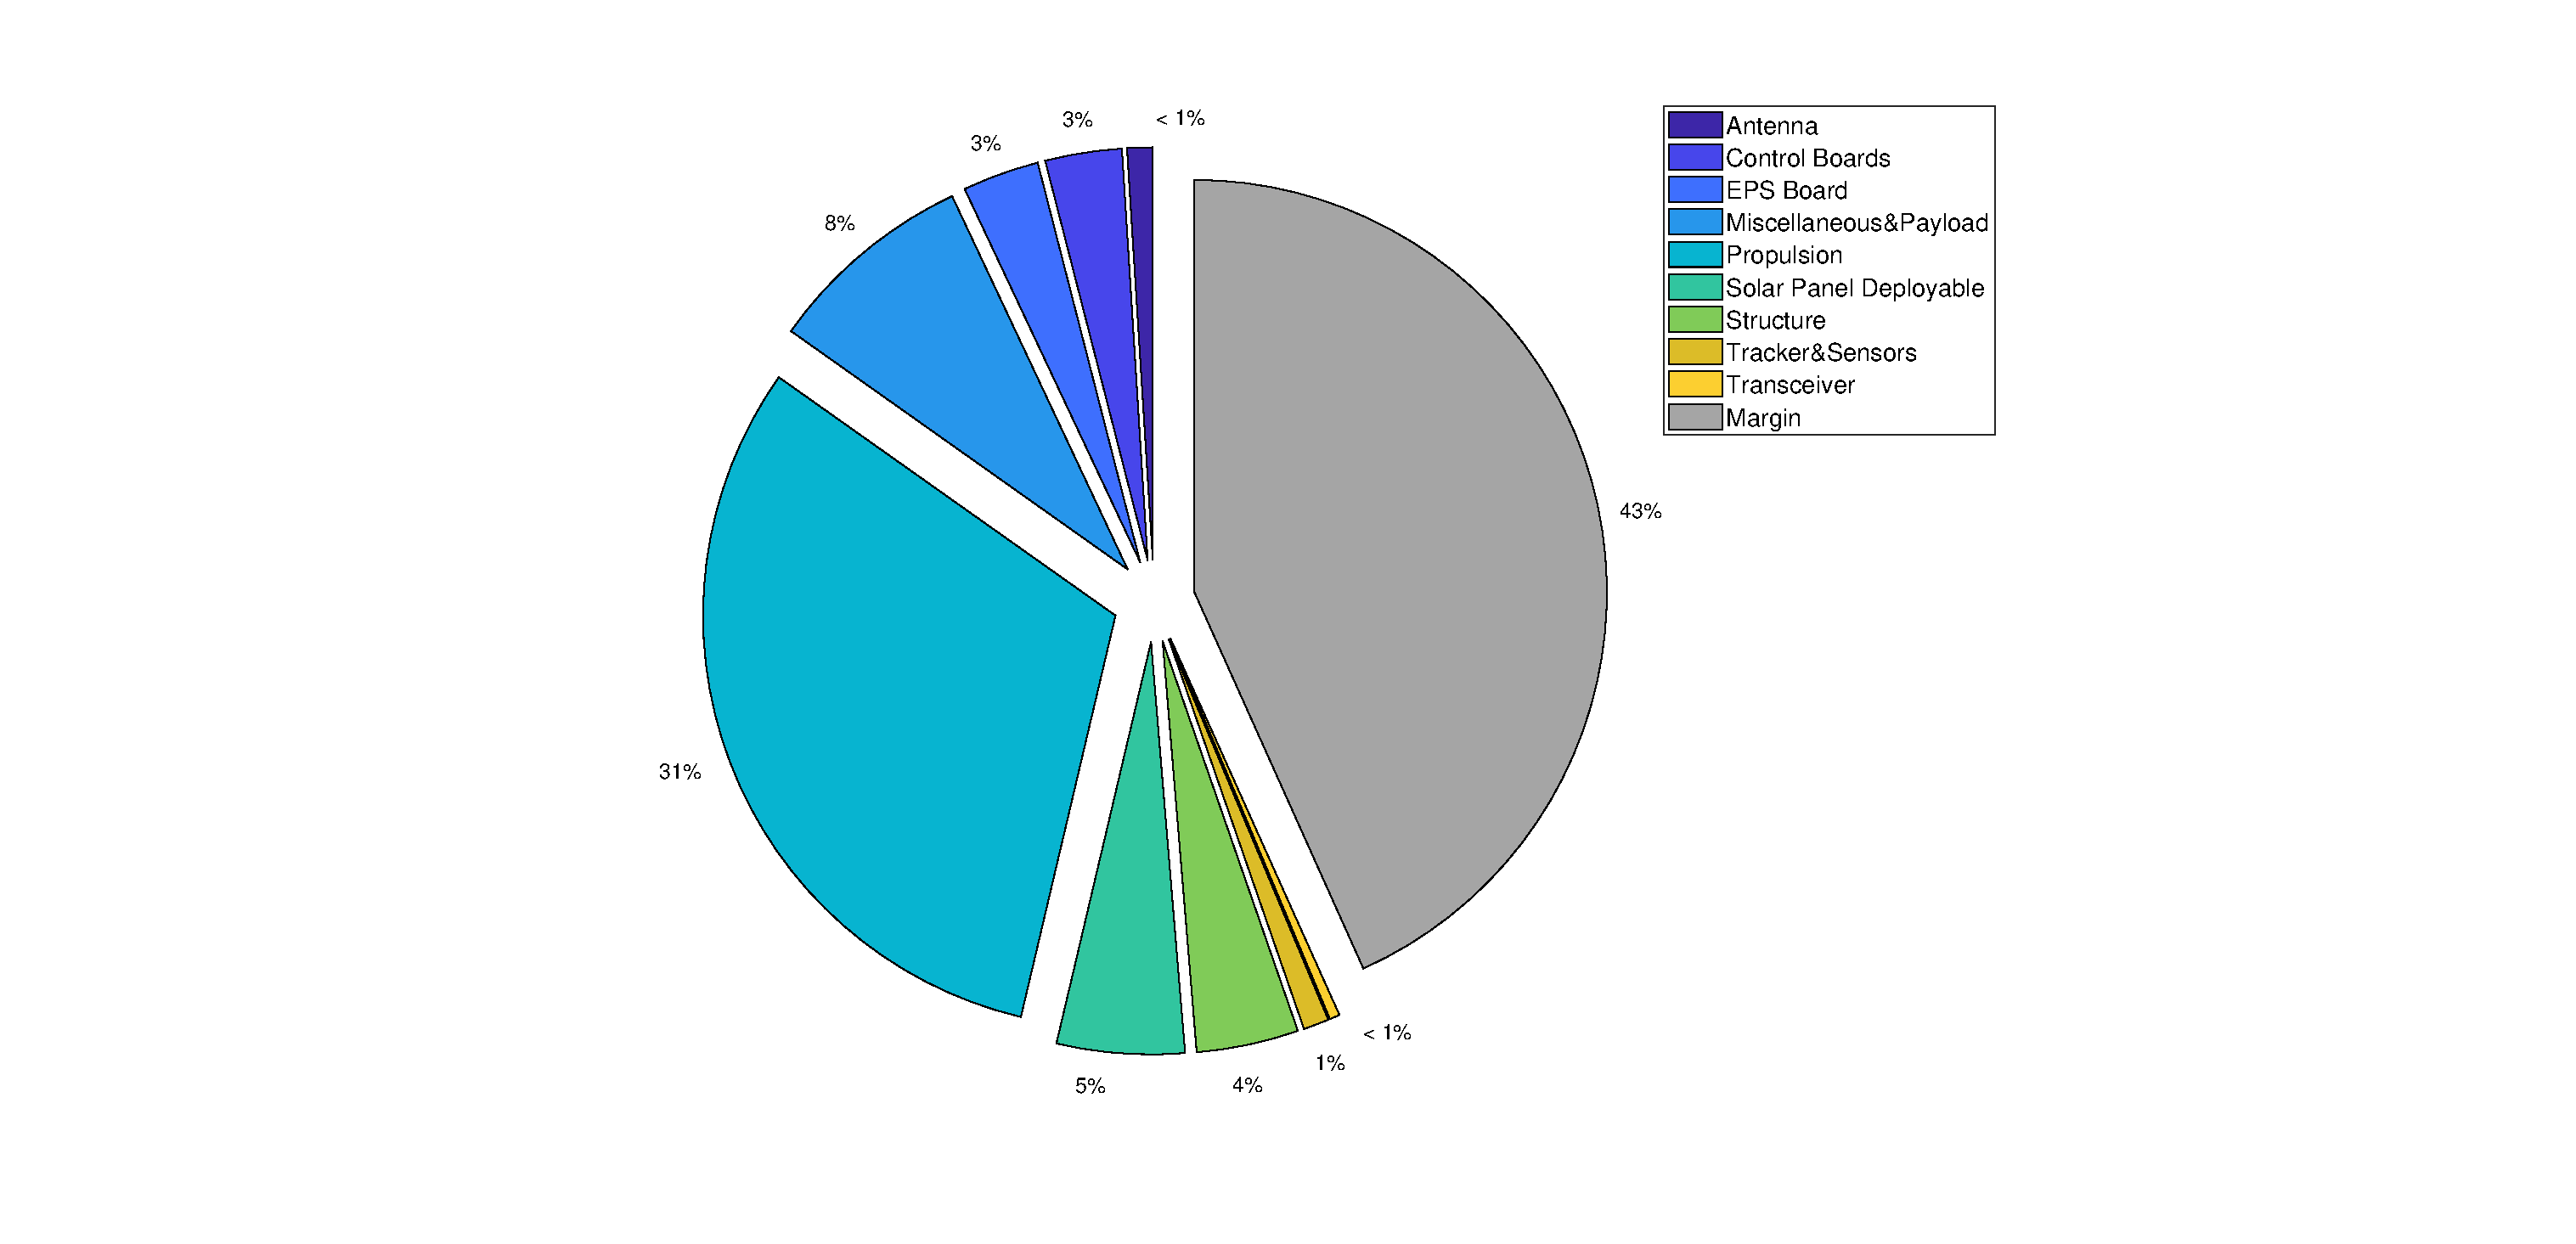
\includegraphics[width=1.00\textwidth]{masse}
											\caption{Massen Budget für das angenommene Design}
											\label{fig:masse}
										\end{figure}
										
						\subsubsection{Volumenbudget}
								
										\begin{figure}[h]
											\centering
												\includegraphics[width=1.00\textwidth]{volume}
											\caption{Volumen Budget für das angenommene Design}
											\label{fig:volume}
										\end{figure}
								
						\subsubsection{Leistungsbudget}
				
			\section{Auswertung und Optimierung des Designs}

				
														% -"- CubeSat Design 														
	\chapter{Auswertung des CubeSat-based ADR Konzepts}

\section{Bewertungsstrategie}
	%Die Strategie besteht draus mehrere Simulationen per GMAT für untershciedliche Koonfigs durchzuführen. Die Bewertung fokusiertsich auf die Machbarkeit des De-orbiting (seihe TODOS.txt)\\
		\subsection{Kriterien der Bewertung}	
		\subsection{GMAT}


\section{Ergebnisse}
		\subsection {Generated Data}
%For every considered satellite design (=mainly thruster configuration, 3-4 different designs), generate following data: \\
%
%Deorbit time and spent fuel mass for all:
%\begin{itemize}
	%\item Masses from 50-500 kg\\
	%\item Altitudes from 1400-400? km  (ggf. semi-major axis) \\
	%\item Eccentricities from ~0 to highest recorded eccentricity of debris in <1400 km orbit
%\end{itemize}
%
%Note: Output EVERY relevant simulation parameter (initial orbit and S/C data, burn start/stop angles, start epoch etc.)  at the beginning of every simulation run [discuss with Max]
	%
			%\subsection{Reachability Enveloppe}
%RESULTING DIAGRAMS: \\
%
%\begin{enumerate}
		%\item Visualize the absolute performance of the main design (Max), e = 0 \\
				%\begin{itemize}
						%\item Axes: y = mass, x = SMA \\
						%\item Graph: Use color gradients to display deorbit times (same time = same color)
				%\end{itemize}
				%\item  Visualize the influence of eccentricity on deorbit times using the main design \\
				%\begin{itemize}
						%\item Axes: y = mass, x = SMA \\
						%\item Select a fixed deorbit time (e.g. 2 years) \\
						%\item Graph: Use color gradients to display eccentricities (same ecc = same color)
				%\end{itemize}
				%\item Visually compare the performances of the different designs (Max \& 2-3 group designs), e = 0 
				%\begin{itemize}
						%\item Axes: y = mass, x = SMA \\
						%\item Select 1-2 fixed deorbit times (e.g. 2 years \& 5 years) \\
						%\item Graph: Draw lines of same deorbit time (selected above) for each of the different designs
				%\end{itemize}				
%\end{enumerate}
%Optional for group after 3. (decide if worth it)\\
%4. Repeat 1. with all other chosen designs\\
%
%NOTES: \\
%
%For 1. \& 4.:\\
%(Deorbit time limited to 10 years (15? 20?)) \\
%-> <2 years of deorbiting takes 3-4 mins to simulate, amount of data is immense => limit maximum deorbit time? \\
%-> At which deorbiting time does a feasible solution become unattractive? If 200 kg in 1000 km orbit is \\
   %deorbitable in 20 years, is it worth it? Better use chemical deorbiting = different mission in this case? \\
%---> Agree on a meaningful limit on deorbit time \\
%
%For all graphs/simulations: \\
%Fuel mass limited by design -> if 27U standard is to be kept no matter which thruster configuration is \\
%chosen, then smaller/more lightweight thrusters would result in more available space for fuel \\
%---> Agree on a set percentage of margin for all designs (e.g. 50\%) and determine maximum fuel from there? \\
%
%-> For Max's design, fuel mass limited to 10 kg (thinking about increasing to 15 kg)\\
			%\subsection{Missionsauslegung}
					%\textbf{Mögliche CubeSat Konfigurationen}\\
			%\subsection{Missionssimulation}
					%\textbf{Impuls-basierter Schub}\\
					%\textbf{Begrenzter Schub}\\
					%\textbf{Mission mit Randbedingungen}\\
			%\subsection{Konfigurationsvergleich}
					%\textbf{..}\\
					%\textbf{..}\\
					%\textbf{..}\\														% -"- Mission Design
  \include{./header_hauptteil/zusammenfassung1}													
  \chapter{Fazit und Ausblick}
Zusammenfassend lässt sich sagen, dass die Simulation der Missionen sehr gut verlaufen ist. Über alle betrachteten Höhen lassen sich, laut der Simulationsergebnisse, defekte Satelliten in der Größenordnung von Megakonstellationen aus der Umlaufbahn entfernen. Entgegen der Erwartungen scheint es sogar möglich zu sein mit dem selben Aufbau deutlich größere Massen abzubremsen. Selbst bei einer Höhe von 1400 $km$ verlief die Simulation mit 475 $kg$ noch erfolgreich. Die derzeit größte bekannte Masse geplanter Megakonstellationssatelliten liegt mit 386 $kg$ deutlich unter diesem Wert \cite{BenLarbi.2017}. Der limitierende Faktor der Mission ist die Treibstoffmenge von 10 $kg$. Eine Testsimulation hat ergeben, dass die Zielgruppe auf größere Massen in hohen Umlaufbahnen erweitert werden kann, wenn die Treibstoffmenge um 50\% erhöht wird. Das wäre zwar innerhalb des Massenbudgets, jedoch ist das Volumen mit der ursprünglichen Auslegung bereits komplett ausgeschöpft. Die Ursache dafür sind unter anderem die Skalierungen der Subsysteme. Des Weiteren müssen die Einbauvorrichtungen der einzelnen Komponenten mit berücksichtigt werden, die bei den Budgets durch das Programm nicht beachtet werden konnten. Zielsetzung der vorliegenden Arbeit war die Eignung des angenommen CubeSat Designs für ADR Missionen zu testen. Da die  Simulationen erfolgreich verlaufen sind benötigt das gewählte Design keine Optimierung. Dies bildet eine gute Voraussetzung für die weiteren Planungen bezüglich der Satellitenkonstellation. Mit diesem Nachweis kann jetzt an dem Wärmemanagement, RCS und Struktur gearbeitet werden, die in dieser Arbeit nur untergeordnet behandelt wurden. Weiterhin wurde festgestellt, dass keine genaue Aussage über die Effizienz des RCS getroffen werden kann, da die RCS-Treibwerksauswahl auf Skalierung basiert. Über sämtliche Komponenten bei denen eine Skalierung stattgefunden hat sollte Rücksprache mit den Herstellern gehalten werden, um möglichst reale Werte für die Berechnungen zur Verfügung zu haben. 

	
	%===================================================
  %
  % Literaturverzeichnis
  %
  %---------------------------------------------------
  \addcontentsline{toc}{chapter}{Literaturverzeichnis}
   \bibliographystyle{ieeetr}
		\bibliography{literaturen}

  
  %===================================================
  %
  % Abbildungsverzeichnis
  %
  %---------------------------------------------------
	\addcontentsline{toc}{chapter}{Abbildungsverzeichnis}
  \listoffigures
  \newpage
  
  %===================================================
  %
  % Tabellenverzeichnis
  %
  %---------------------------------------------------
	\addcontentsline{toc}{chapter}{Tabellenverzeichnis}
		\listoftables																										% Tabellenverzeichnis
			\newpage
  
  %===================================================
  %
  % Symbol- und Abkürzungsverzeichnis
  %
  %---------------------------------------------------
 \chapter*{Symbolverzeichnis}																					% Symbolverzeichnis
   \addcontentsline{toc}{chapter}{Symbolverzeichnis}									% fügt Symbolverzeichnis trotz * in das Inhaltsverzeichnis ein
        \printglossary[type=symbolslist, title=Symbole und Indizes]		% symbols
   \printglossary[type=acronymlist, title=Abk\"urzungen]							% abbreviations
 \glsaddall 
  \newpage
	
  %===================================================
  %
  % Anhang
  %
  %---------------------------------
		\begin{appendix}
			\chapter{Projektmanagement}
\label{cha:projekt}
%---------------------------------------- WBS beginnt -----------------------------------------------------------
\section{Work Breakdown Structure}
\label{sec:wbs}

\begin{landscape}
\begin{tikzpicture}[
  basic/.style   = {draw, text width=2.7cm, align=left, drop shadow, rectangle},
  root/.style    = {basic, text width=12cm, rounded corners=2pt, thin, align=center, fill=gray90},
  level 2/.style = {basic, rounded corners=2pt, thin, fill=gray80},
  level 3/.style = {basic, thin, fill=gray90, text width=2.6cm},
  level 1/.style={sibling distance=38mm}, edge from parent fork down, 
  edge from parent/.style={->,draw}, level distance=2.5cm,  >=latex]

% root of the the initial tree, level 1
\node[root] {\tb{Analyse einer CubeSat basierenden ADR-Mission}}
% The first level, as children of the initial tree
  child {node[level 2] (c1) {\tb{AP~1000} \\ Literatur-recherche}}
  child {node[level 2] (c2) {\tb{AP~2000} \\ CubeSat Design}}
  child {node[level 2] (c3) {\tb{AP~3000} \\ Budgetplanung mit QuSad}}
  child {node[level 2] (c4) {\tb{AP~4000} \\ Missions-planung mit GMat}}
  child {node[level 2] (c5) {\tb{AP~5000} \\ Dokumentation \\ $~~$}};

% The second level, relatively positioned nodes
\begin{scope}[every node/.style={level 3}, node distance=6pt]
\node [below=of c1, xshift=10pt] (c11) {\tb{AP~1100} \\ Weltraumm\"ull-problematik};
\node [below=of c11] (c12) {\tb{AP~1200} \\ CubeSat Subsysteme};
\node [below=of c12] (c13) {\tb{AP~1300} \\ Rendezvou und Docking};
\node [below=of c13] (c14) {\tb{AP~1400} \\ Erforderliche Softwares};


\node [below=of c2, xshift=10pt] (c21) {\tb{AP~2100} \\ CubeSat Datenbank Analyse};
\node [below=of c21] (c22) {\tb{AP~2200} \\ Ausarbeitung von effizienten Subsystemen};
\node [below=of c22] (c23) {\tb{AP~2300} \\ Ausarbeitung von CubeSat Konfigurationen};

\node [below=of c3, xshift=10pt] (c31) {\tb{AP~3100} \\ Datenbank-erweiterung};
\node [below=of c31] (c32) {\tb{AP~3200} \\ Generierung der CubeSat Konfigurationen};
\node [below=of c32] (c33) {\tb{AP~3300} \\ Budget-kalkulation und Vergleich};

\node [below=of c4, xshift=10pt] (c41) {\tb{AP~4100} \\ Missions-auslegung};
\node [below=of c41] (c42) {\tb{AP~4200} \\ Durchführung der Simulation};
\node [below=of c42] (c43) {\tb{AP~4300} \\ Auswertung der Simulation};

\node [below=of c5, xshift=10pt] (c51) {\tb{AP~5100} \\ Textverfassung};
\node [below=of c51] (c52) {\tb{AP~5200} \\ Überprüfung};

\end{scope}
%--------------------------------------------- Pfeile für das Diagramm vom WBS -------------------------------------
%-----------------------------------lines from each level 1 node to every one of its "children"--------------------
\foreach \value in {1,2,3,4}
  \draw[->] (c1.212) |- (c1\value.west);

\foreach \value in {1,2,3}
  \draw[->] (c2.212) |- (c2\value.west);

\foreach \value in {1,2,3}
  \draw[->] (c3.212) |- (c3\value.west);

\foreach \value in {1,2,3}
  \draw[->] (c4.212) |- (c4\value.west);

\foreach \value in {1,2}
  \draw[->] (c5.212) |- (c5\value.west);
  
\end{tikzpicture}
\end{landscape}

\section{Zeitplan}
\label{sec:zeitplan}
%----------------------------------------------- Ganttchart Diagramm -----------------------------------------------
\begin{landscape}
%\noindent\resizebox{\textwidth}{!}{	% Einfügen, falls zu groß
\begin{ganttchart}[hgrid,
                   time slot format = isodate, 
                   x unit=0.28cm,	% Zum komprimieren des Charts in x-Richtung
                   %y unit chart=0.7cm,
                   %compress calendar,	% Komprimiert den Chart in der Breite
                   calendar week text = {Woche~\currentweek},
                   chart element start border = right,
                   bar/.append style={fill=blue!40, rounded corners=2pt},
                   bar incomplete/.append style={fill=blue!10},
                   bar label node/.append style={align=left, text width=7cm},
                   group label node/.append style={align=left, text width=8cm},
                   milestone label node/.append style={align=left, text width=8cm},
                   bar progress label node/.style={right=2mm},
                   progress label text = {\pgfmathprintnumber[precision=0, verbatim]{#1}\%},
                  ]{2013-01-01}{2013-02-23}
  \gantttitlecalendar{year, month=shortname, week}\\
  %\gantttitle{2013}{59}\\
  \ganttgroup{AP 1000: Literaturrecherche}{2013-01-01}{2013-02-01}\\
  \ganttbar[progress=50]  {AP 1100: Weltraummüllproblematik}{2013-01-01}{2013-01-08}\\
  \ganttlinkedbar {AP 1200: Beobachtung von Weltraummüll}{2013-01-09}{2013-01-17}\\
  \ganttlinkedbar {AP 1300: Bahnbestimmung mit optischen Sensoren}{2013-01-17}{2013-02-01}\\
  %\ganttbar[progress=100]{AP 1300: TEXT}{2013-01-01}{2013-01-30}\\	% Beispiel für Fortschrittsbalken!
  
  \ganttgroup{AP 2000: Algorithmuserstellung}{2013-02-02}{2013-02-23}\\
  \ganttbar  {AP 2100: ...}{2013-02-02}{2013-02-09}\\
  \ganttbar  {AP 2200: ...}{2013-02-10}{2013-02-19}\\
  
  \ganttmilestone{Meilenstein}{2013-02-20}\\
  
 \end{ganttchart}
%}
\end{landscape}

\section{Work Package Description}
\label{sec:wpd}


%--------------------------------------------- AP Literaturrecherche ------------------------------------------
%-------------------------------------------- Tabelle Weltraummüllproblematik ---------------------------------
\begin{table}[!h]
 \begin{center}
  \begin{tabular}{|p{35mm}||p{55mm}|p{50mm}||p{40mm}|}
   \hline
   \multicolumn{3}{|l||}{\textbf{}} & \multicolumn{1}{c|}{}\\
   \multicolumn{3}{|l||}{\textbf{}} & \multicolumn{1}{c|}{\textbf{AP 1100}}\\
   \multicolumn{3}{|l||}{\textbf{}} & \multicolumn{1}{c|}{}\\
   \hline\hline
   \textbf{Titel} & \multicolumn{2}{p{7cm}||}{\textbf{Weltraummüllproblematik}} & \textbf{Seite:} X von Y\\
   \hline
   \textbf{Verantwortlicher} & \multicolumn{2}{l||}{Dein Name} & \textbf{Version:} 1.1\\
   \hline
   \multicolumn{3}{|l||}{} & \textbf{Datum:} 00.00.2019\\
   \hline\hline
   \textbf{Beginn} & \multicolumn{2}{l||}{T$_0$} & \\
   \hline
   \textbf{Ende} & \multicolumn{2}{l||}{T$_0$+X Wochen} & \textbf{Dauer}: X Wochen\\
   \hline\hline
   \textbf{Bearbeiter} & \multicolumn{3}{l|}{Dein Name}\\
   \hline\hline
   \multicolumn{4}{|p{150mm}|}{\textbf{Ziele:}}\\
   \multicolumn{4}{|p{150mm}|}{$\bullet$ Ziel 1}\\
   \multicolumn{4}{|p{150mm}|}{$\bullet$ Ziel 2}\\
   \multicolumn{4}{|p{150mm}|}{$\bullet$ ...}\\
   \multicolumn{4}{|p{150mm}|}{}\\
   \multicolumn{4}{|p{150mm}|}{\textbf{Input:}}\\
   \multicolumn{4}{|p{150mm}|}{$\bullet$ Input 1}\\
   \multicolumn{4}{|p{150mm}|}{$\bullet$ ...}\\
   \multicolumn{4}{|p{150mm}|}{}\\
   \multicolumn{4}{|p{150mm}|}{\textbf{Schnittstellen zu anderen APs:}}\\
   \multicolumn{4}{|p{150mm}|}{$\bullet$ \textbf{AP XXXX} Beschreibung}\\
   \multicolumn{4}{|p{150mm}|}{$\bullet$ \textbf{AP ....} ...}\\
   \multicolumn{4}{|p{150mm}|}{}\\
   \multicolumn{4}{|p{150mm}|}{\textbf{Aufgaben:}}\\
   \multicolumn{4}{|p{150mm}|}{$\bullet$ Aufgabe 1}\\
   \multicolumn{4}{|p{150mm}|}{$\bullet$ ...}\\
   \multicolumn{4}{|p{150mm}|}{}\\
   \multicolumn{4}{|p{150mm}|}{\textbf{Ergebnisse:}}\\
   \multicolumn{4}{|p{150mm}|}{$\bullet$ Ergebnis 1}\\
   \multicolumn{4}{|p{150mm}|}{$\bullet$ ...}\\
   \hline
  \end{tabular}
 \end{center}
\end{table}

\clearpage
%-------------------------------------------- Tabelle CubeSat Subsysteme ----------------------------------------
\begin{table}[!h]
 \begin{center}
  \begin{tabular}{|p{35mm}||p{55mm}|p{50mm}||p{40mm}|}
   \hline
   \multicolumn{3}{|l||}{\textbf{}} & \multicolumn{1}{c|}{}\\
   \multicolumn{3}{|l||}{\textbf{}} & \multicolumn{1}{c|}{\textbf{AP 1200}}\\
   \multicolumn{3}{|l||}{\textbf{}} & \multicolumn{1}{c|}{}\\
   \hline\hline
   \textbf{Titel} & \multicolumn{2}{p{7cm}||}{\textbf{CubeSat Subsysteme}} & \textbf{Seite:} X von Y\\
   \hline
   \textbf{Verantwortlicher} & \multicolumn{2}{l||}{Dein Name} & \textbf{Version:} 1.1\\
   \hline
   \multicolumn{3}{|l||}{} & \textbf{Datum:} 00.00.2019\\
   \hline\hline
   \textbf{Beginn} & \multicolumn{2}{l||}{T$_0$} & \\
   \hline
   \textbf{Ende} & \multicolumn{2}{l||}{T$_0$+X Wochen} & \textbf{Dauer}: X Wochen\\
   \hline\hline
   \textbf{Bearbeiter} & \multicolumn{3}{l|}{Dein Name}\\
   \hline\hline
   \multicolumn{4}{|p{150mm}|}{\textbf{Ziele:}}\\
   \multicolumn{4}{|p{150mm}|}{$\bullet$ Ziel 1}\\
   \multicolumn{4}{|p{150mm}|}{$\bullet$ Ziel 2}\\
   \multicolumn{4}{|p{150mm}|}{$\bullet$ ...}\\
   \multicolumn{4}{|p{150mm}|}{}\\
   \multicolumn{4}{|p{150mm}|}{\textbf{Input:}}\\
   \multicolumn{4}{|p{150mm}|}{$\bullet$ Input 1}\\
   \multicolumn{4}{|p{150mm}|}{$\bullet$ ...}\\
   \multicolumn{4}{|p{150mm}|}{}\\
   \multicolumn{4}{|p{150mm}|}{\textbf{Schnittstellen zu anderen APs:}}\\
   \multicolumn{4}{|p{150mm}|}{$\bullet$ \textbf{AP XXXX} Beschreibung}\\
   \multicolumn{4}{|p{150mm}|}{$\bullet$ \textbf{AP ....} ...}\\
   \multicolumn{4}{|p{150mm}|}{}\\
   \multicolumn{4}{|p{150mm}|}{\textbf{Aufgaben:}}\\
   \multicolumn{4}{|p{150mm}|}{$\bullet$ Aufgabe 1}\\
   \multicolumn{4}{|p{150mm}|}{$\bullet$ ...}\\
   \multicolumn{4}{|p{150mm}|}{}\\
   \multicolumn{4}{|p{150mm}|}{\textbf{Ergebnisse:}}\\
   \multicolumn{4}{|p{150mm}|}{$\bullet$ Ergebnis 1}\\
   \multicolumn{4}{|p{150mm}|}{$\bullet$ ...}\\
   \hline
  \end{tabular}
 \end{center}
\end{table}

\clearpage
%-------------------------------------------- Tabelle Rendezvous und Docking -------------------------------
\begin{table}[!h]
 \begin{center}
  \begin{tabular}{|p{35mm}||p{55mm}|p{50mm}||p{40mm}|}
   \hline
   \multicolumn{3}{|l||}{\textbf{}} & \multicolumn{1}{c|}{}\\
   \multicolumn{3}{|l||}{\textbf{}} & \multicolumn{1}{c|}{\textbf{AP 1300}}\\
   \multicolumn{3}{|l||}{\textbf{}} & \multicolumn{1}{c|}{}\\
   \hline\hline
   \textbf{Titel} & \multicolumn{2}{p{7cm}||}{\textbf{Rendezvous und Docking}} & \textbf{Seite:} X von Y\\
   \hline
   \textbf{Verantwortlicher} & \multicolumn{2}{l||}{Dein Name} & \textbf{Version:} 1.1\\
   \hline
   \multicolumn{3}{|l||}{} & \textbf{Datum:} 00.00.2019\\
   \hline\hline
   \textbf{Beginn} & \multicolumn{2}{l||}{T$_0$} & \\
   \hline
   \textbf{Ende} & \multicolumn{2}{l||}{T$_0$+X Wochen} & \textbf{Dauer}: X Wochen\\
   \hline\hline
   \textbf{Bearbeiter} & \multicolumn{3}{l|}{Dein Name}\\
   \hline\hline
   \multicolumn{4}{|p{150mm}|}{\textbf{Ziele:}}\\
   \multicolumn{4}{|p{150mm}|}{$\bullet$ Ziel 1}\\
   \multicolumn{4}{|p{150mm}|}{$\bullet$ Ziel 2}\\
   \multicolumn{4}{|p{150mm}|}{$\bullet$ ...}\\
   \multicolumn{4}{|p{150mm}|}{}\\
   \multicolumn{4}{|p{150mm}|}{\textbf{Input:}}\\
   \multicolumn{4}{|p{150mm}|}{$\bullet$ Input 1}\\
   \multicolumn{4}{|p{150mm}|}{$\bullet$ ...}\\
   \multicolumn{4}{|p{150mm}|}{}\\
   \multicolumn{4}{|p{150mm}|}{\textbf{Schnittstellen zu anderen APs:}}\\
   \multicolumn{4}{|p{150mm}|}{$\bullet$ \textbf{AP XXXX} Beschreibung}\\
   \multicolumn{4}{|p{150mm}|}{$\bullet$ \textbf{AP ....} ...}\\
   \multicolumn{4}{|p{150mm}|}{}\\
   \multicolumn{4}{|p{150mm}|}{\textbf{Aufgaben:}}\\
   \multicolumn{4}{|p{150mm}|}{$\bullet$ Aufgabe 1}\\
   \multicolumn{4}{|p{150mm}|}{$\bullet$ ...}\\
   \multicolumn{4}{|p{150mm}|}{}\\
   \multicolumn{4}{|p{150mm}|}{\textbf{Ergebnisse:}}\\
   \multicolumn{4}{|p{150mm}|}{$\bullet$ Ergebnis 1}\\
   \multicolumn{4}{|p{150mm}|}{$\bullet$ ...}\\
   \hline
  \end{tabular}
 \end{center}
\end{table}

\clearpage
%-------------------------------------------- Tabelle Erforderliche Software ------------------------------
\begin{table}[!h]
 \begin{center}
  \begin{tabular}{|p{35mm}||p{55mm}|p{50mm}||p{40mm}|}
   \hline
   \multicolumn{3}{|l||}{\textbf{}} & \multicolumn{1}{c|}{}\\
   \multicolumn{3}{|l||}{\textbf{}} & \multicolumn{1}{c|}{\textbf{AP 1400}}\\
   \multicolumn{3}{|l||}{\textbf{}} & \multicolumn{1}{c|}{}\\
   \hline\hline
   \textbf{Titel} & \multicolumn{2}{p{7cm}||}{\textbf{Software}} & \textbf{Seite:} X von Y\\
   \hline
   \textbf{Verantwortlicher} & \multicolumn{2}{l||}{Dein Name} & \textbf{Version:} 1.1\\
   \hline
   \multicolumn{3}{|l||}{} & \textbf{Datum:} 00.00.2019\\
   \hline\hline
   \textbf{Beginn} & \multicolumn{2}{l||}{T$_0$} & \\
   \hline
   \textbf{Ende} & \multicolumn{2}{l||}{T$_0$+X Wochen} & \textbf{Dauer}: X Wochen\\
   \hline\hline
   \textbf{Bearbeiter} & \multicolumn{3}{l|}{Dein Name}\\
   \hline\hline
   \multicolumn{4}{|p{150mm}|}{\textbf{Ziele:}}\\
   \multicolumn{4}{|p{150mm}|}{$\bullet$ Ziel 1}\\
   \multicolumn{4}{|p{150mm}|}{$\bullet$ Ziel 2}\\
   \multicolumn{4}{|p{150mm}|}{$\bullet$ ...}\\
   \multicolumn{4}{|p{150mm}|}{}\\
   \multicolumn{4}{|p{150mm}|}{\textbf{Input:}}\\
   \multicolumn{4}{|p{150mm}|}{$\bullet$ Input 1}\\
   \multicolumn{4}{|p{150mm}|}{$\bullet$ ...}\\
   \multicolumn{4}{|p{150mm}|}{}\\
   \multicolumn{4}{|p{150mm}|}{\textbf{Schnittstellen zu anderen APs:}}\\
   \multicolumn{4}{|p{150mm}|}{$\bullet$ \textbf{AP XXXX} Beschreibung}\\
   \multicolumn{4}{|p{150mm}|}{$\bullet$ \textbf{AP ....} ...}\\
   \multicolumn{4}{|p{150mm}|}{}\\
   \multicolumn{4}{|p{150mm}|}{\textbf{Aufgaben:}}\\
   \multicolumn{4}{|p{150mm}|}{$\bullet$ Aufgabe 1}\\
   \multicolumn{4}{|p{150mm}|}{$\bullet$ ...}\\
   \multicolumn{4}{|p{150mm}|}{}\\
   \multicolumn{4}{|p{150mm}|}{\textbf{Ergebnisse:}}\\
   \multicolumn{4}{|p{150mm}|}{$\bullet$ Ergebnis 1}\\
   \multicolumn{4}{|p{150mm}|}{$\bullet$ ...}\\
   \hline
  \end{tabular}
 \end{center}
\end{table}

\clearpage
%-------------------------------------------- AP Cubesat Design -----------------------------------------------
%------------------------------------ Tabelle CubeSat Datenbank Analyse ---------------------------------------
\begin{table}[!h]
 \begin{center}
  \begin{tabular}{|p{35mm}||p{55mm}|p{50mm}||p{40mm}|}
   \hline
   \multicolumn{3}{|l||}{\textbf{}} & \multicolumn{1}{c|}{}\\
   \multicolumn{3}{|l||}{\textbf{}} & \multicolumn{1}{c|}{\textbf{AP 2100}}\\
   \multicolumn{3}{|l||}{\textbf{}} & \multicolumn{1}{c|}{}\\
   \hline\hline
   \textbf{Titel} & \multicolumn{2}{p{7cm}||}{\textbf{CubeSat Datenbank Analyse}} & \textbf{Seite:} X von Y\\
   \hline
   \textbf{Verantwortlicher} & \multicolumn{2}{l||}{Dein Name} & \textbf{Version:} 1.1\\
   \hline
   \multicolumn{3}{|l||}{} & \textbf{Datum:} 00.00.2019\\
   \hline\hline
   \textbf{Beginn} & \multicolumn{2}{l||}{T$_0$} & \\
   \hline
   \textbf{Ende} & \multicolumn{2}{l||}{T$_0$+X Wochen} & \textbf{Dauer}: X Wochen\\
   \hline\hline
   \textbf{Bearbeiter} & \multicolumn{3}{l|}{Dein Name}\\
   \hline\hline
   \multicolumn{4}{|p{150mm}|}{\textbf{Ziele:}}\\
   \multicolumn{4}{|p{150mm}|}{$\bullet$ Ziel 1}\\
   \multicolumn{4}{|p{150mm}|}{$\bullet$ Ziel 2}\\
   \multicolumn{4}{|p{150mm}|}{$\bullet$ ...}\\
   \multicolumn{4}{|p{150mm}|}{}\\
   \multicolumn{4}{|p{150mm}|}{\textbf{Input:}}\\
   \multicolumn{4}{|p{150mm}|}{$\bullet$ Input 1}\\
   \multicolumn{4}{|p{150mm}|}{$\bullet$ ...}\\
   \multicolumn{4}{|p{150mm}|}{}\\
   \multicolumn{4}{|p{150mm}|}{\textbf{Schnittstellen zu anderen APs:}}\\
   \multicolumn{4}{|p{150mm}|}{$\bullet$ \textbf{AP XXXX} Beschreibung}\\
   \multicolumn{4}{|p{150mm}|}{$\bullet$ \textbf{AP ....} ...}\\
   \multicolumn{4}{|p{150mm}|}{}\\
   \multicolumn{4}{|p{150mm}|}{\textbf{Aufgaben:}}\\
   \multicolumn{4}{|p{150mm}|}{$\bullet$ Aufgabe 1}\\
   \multicolumn{4}{|p{150mm}|}{$\bullet$ ...}\\
   \multicolumn{4}{|p{150mm}|}{}\\
   \multicolumn{4}{|p{150mm}|}{\textbf{Ergebnisse:}}\\
   \multicolumn{4}{|p{150mm}|}{$\bullet$ Ergebnis 1}\\
   \multicolumn{4}{|p{150mm}|}{$\bullet$ ...}\\
   \hline
  \end{tabular}
 \end{center}
\end{table}

\clearpage
%------------------------------------ Tabelle Ausarbeitung von effizienten Subsystemen -------------------------------------
\begin{table}[!h]
 \begin{center}
  \begin{tabular}{|p{35mm}||p{55mm}|p{50mm}||p{40mm}|}
   \hline
   \multicolumn{3}{|l||}{\textbf{}} & \multicolumn{1}{c|}{}\\
   \multicolumn{3}{|l||}{\textbf{}} & \multicolumn{1}{c|}{\textbf{AP 2200}}\\
   \multicolumn{3}{|l||}{\textbf{}} & \multicolumn{1}{c|}{}\\
   \hline\hline
   \textbf{Titel} & \multicolumn{2}{p{7cm}||}{\textbf{Ausarbeitung von effizienten Subsystemen}} & \textbf{Seite:} X von Y\\
   \hline
   \textbf{Verantwortlicher} & \multicolumn{2}{l||}{Dein Name} & \textbf{Version:} 1.1\\
   \hline
   \multicolumn{3}{|l||}{} & \textbf{Datum:} 00.00.2019\\
   \hline\hline
   \textbf{Beginn} & \multicolumn{2}{l||}{T$_0$} & \\
   \hline
   \textbf{Ende} & \multicolumn{2}{l||}{T$_0$+X Wochen} & \textbf{Dauer}: X Wochen\\
   \hline\hline
   \textbf{Bearbeiter} & \multicolumn{3}{l|}{Dein Name}\\
   \hline\hline
   \multicolumn{4}{|p{150mm}|}{\textbf{Ziele:}}\\
   \multicolumn{4}{|p{150mm}|}{$\bullet$ Ziel 1}\\
   \multicolumn{4}{|p{150mm}|}{$\bullet$ Ziel 2}\\
   \multicolumn{4}{|p{150mm}|}{$\bullet$ ...}\\
   \multicolumn{4}{|p{150mm}|}{}\\
   \multicolumn{4}{|p{150mm}|}{\textbf{Input:}}\\
   \multicolumn{4}{|p{150mm}|}{$\bullet$ Input 1}\\
   \multicolumn{4}{|p{150mm}|}{$\bullet$ ...}\\
   \multicolumn{4}{|p{150mm}|}{}\\
   \multicolumn{4}{|p{150mm}|}{\textbf{Schnittstellen zu anderen APs:}}\\
   \multicolumn{4}{|p{150mm}|}{$\bullet$ \textbf{AP XXXX} Beschreibung}\\
   \multicolumn{4}{|p{150mm}|}{$\bullet$ \textbf{AP ....} ...}\\
   \multicolumn{4}{|p{150mm}|}{}\\
   \multicolumn{4}{|p{150mm}|}{\textbf{Aufgaben:}}\\
   \multicolumn{4}{|p{150mm}|}{$\bullet$ Aufgabe 1}\\
   \multicolumn{4}{|p{150mm}|}{$\bullet$ ...}\\
   \multicolumn{4}{|p{150mm}|}{}\\
   \multicolumn{4}{|p{150mm}|}{\textbf{Ergebnisse:}}\\
   \multicolumn{4}{|p{150mm}|}{$\bullet$ Ergebnis 1}\\
   \multicolumn{4}{|p{150mm}|}{$\bullet$ ...}\\
   \hline
  \end{tabular}
 \end{center}
\end{table}

\clearpage
%----------------------------------- Tabelle Ausarbeitung von CubeSat Konfigurationen ----------------------------------------
\begin{table}[!h]
 \begin{center}
  \begin{tabular}{|p{35mm}||p{55mm}|p{50mm}||p{40mm}|}
   \hline
   \multicolumn{3}{|l||}{\textbf{}} & \multicolumn{1}{c|}{}\\
   \multicolumn{3}{|l||}{\textbf{}} & \multicolumn{1}{c|}{\textbf{AP 2300}}\\
   \multicolumn{3}{|l||}{\textbf{}} & \multicolumn{1}{c|}{}\\
   \hline\hline
   \textbf{Titel} & \multicolumn{2}{p{7cm}||}{\textbf{Ausarbeitung von CubeSat Konfigurationen}} & \textbf{Seite:} X von Y\\
   \hline
   \textbf{Verantwortlicher} & \multicolumn{2}{l||}{Dein Name} & \textbf{Version:} 1.1\\
   \hline
   \multicolumn{3}{|l||}{} & \textbf{Datum:} 00.00.2019\\
   \hline\hline
   \textbf{Beginn} & \multicolumn{2}{l||}{T$_0$} & \\
   \hline
   \textbf{Ende} & \multicolumn{2}{l||}{T$_0$+X Wochen} & \textbf{Dauer}: X Wochen\\
   \hline\hline
   \textbf{Bearbeiter} & \multicolumn{3}{l|}{Dein Name}\\
   \hline\hline
   \multicolumn{4}{|p{150mm}|}{\textbf{Ziele:}}\\
   \multicolumn{4}{|p{150mm}|}{$\bullet$ Ziel 1}\\
   \multicolumn{4}{|p{150mm}|}{$\bullet$ Ziel 2}\\
   \multicolumn{4}{|p{150mm}|}{$\bullet$ ...}\\
   \multicolumn{4}{|p{150mm}|}{}\\
   \multicolumn{4}{|p{150mm}|}{\textbf{Input:}}\\
   \multicolumn{4}{|p{150mm}|}{$\bullet$ Input 1}\\
   \multicolumn{4}{|p{150mm}|}{$\bullet$ ...}\\
   \multicolumn{4}{|p{150mm}|}{}\\
   \multicolumn{4}{|p{150mm}|}{\textbf{Schnittstellen zu anderen APs:}}\\
   \multicolumn{4}{|p{150mm}|}{$\bullet$ \textbf{AP XXXX} Beschreibung}\\
   \multicolumn{4}{|p{150mm}|}{$\bullet$ \textbf{AP ....} ...}\\
   \multicolumn{4}{|p{150mm}|}{}\\
   \multicolumn{4}{|p{150mm}|}{\textbf{Aufgaben:}}\\
   \multicolumn{4}{|p{150mm}|}{$\bullet$ Aufgabe 1}\\
   \multicolumn{4}{|p{150mm}|}{$\bullet$ ...}\\
   \multicolumn{4}{|p{150mm}|}{}\\
   \multicolumn{4}{|p{150mm}|}{\textbf{Ergebnisse:}}\\
   \multicolumn{4}{|p{150mm}|}{$\bullet$ Ergebnis 1}\\
   \multicolumn{4}{|p{150mm}|}{$\bullet$ ...}\\
   \hline
  \end{tabular}
 \end{center}
\end{table}

\clearpage
%----------------------------------------- AP Budgetplanung mit QuSad -----------------------------------------
%----------------------------------------- Tabelle Datenbankerweiterung ---------------------------------------
\begin{table}[!h]
 \begin{center}
  \begin{tabular}{|p{35mm}||p{55mm}|p{50mm}||p{40mm}|}
   \hline
   \multicolumn{3}{|l||}{\textbf{}} & \multicolumn{1}{c|}{}\\
   \multicolumn{3}{|l||}{\textbf{}} & \multicolumn{1}{c|}{\textbf{AP 3100}}\\
   \multicolumn{3}{|l||}{\textbf{}} & \multicolumn{1}{c|}{}\\
   \hline\hline
   \textbf{Titel} & \multicolumn{2}{p{7cm}||}{\textbf{Datenbankerweiterung}} & \textbf{Seite:} X von Y\\
   \hline
   \textbf{Verantwortlicher} & \multicolumn{2}{l||}{Dein Name} & \textbf{Version:} 1.1\\
   \hline
   \multicolumn{3}{|l||}{} & \textbf{Datum:} 00.00.2019\\
   \hline\hline
   \textbf{Beginn} & \multicolumn{2}{l||}{T$_0$} & \\
   \hline
   \textbf{Ende} & \multicolumn{2}{l||}{T$_0$+X Wochen} & \textbf{Dauer}: X Wochen\\
   \hline\hline
   \textbf{Bearbeiter} & \multicolumn{3}{l|}{Dein Name}\\
   \hline\hline
   \multicolumn{4}{|p{150mm}|}{\textbf{Ziele:}}\\
   \multicolumn{4}{|p{150mm}|}{$\bullet$ Ziel 1}\\
   \multicolumn{4}{|p{150mm}|}{$\bullet$ Ziel 2}\\
   \multicolumn{4}{|p{150mm}|}{$\bullet$ ...}\\
   \multicolumn{4}{|p{150mm}|}{}\\
   \multicolumn{4}{|p{150mm}|}{\textbf{Input:}}\\
   \multicolumn{4}{|p{150mm}|}{$\bullet$ Input 1}\\
   \multicolumn{4}{|p{150mm}|}{$\bullet$ ...}\\
   \multicolumn{4}{|p{150mm}|}{}\\
   \multicolumn{4}{|p{150mm}|}{\textbf{Schnittstellen zu anderen APs:}}\\
   \multicolumn{4}{|p{150mm}|}{$\bullet$ \textbf{AP XXXX} Beschreibung}\\
   \multicolumn{4}{|p{150mm}|}{$\bullet$ \textbf{AP ....} ...}\\
   \multicolumn{4}{|p{150mm}|}{}\\
   \multicolumn{4}{|p{150mm}|}{\textbf{Aufgaben:}}\\
   \multicolumn{4}{|p{150mm}|}{$\bullet$ Aufgabe 1}\\
   \multicolumn{4}{|p{150mm}|}{$\bullet$ ...}\\
   \multicolumn{4}{|p{150mm}|}{}\\
   \multicolumn{4}{|p{150mm}|}{\textbf{Ergebnisse:}}\\
   \multicolumn{4}{|p{150mm}|}{$\bullet$ Ergebnis 1}\\
   \multicolumn{4}{|p{150mm}|}{$\bullet$ ...}\\
   \hline
  \end{tabular}
 \end{center}
\end{table}

\clearpage
%--------------------------------------- Tabelle Generierung der CubeSat Konfigurationen -----------------------------------
\begin{table}[!h]
 \begin{center}
  \begin{tabular}{|p{35mm}||p{55mm}|p{50mm}||p{40mm}|}
   \hline
   \multicolumn{3}{|l||}{\textbf{}} & \multicolumn{1}{c|}{}\\
   \multicolumn{3}{|l||}{\textbf{}} & \multicolumn{1}{c|}{\textbf{AP 3200}}\\
   \multicolumn{3}{|l||}{\textbf{}} & \multicolumn{1}{c|}{}\\
   \hline\hline
   \textbf{Titel} & \multicolumn{2}{p{7cm}||}{\textbf{Generierung der CubeSat Konfigurationen}} & \textbf{Seite:} X von Y\\
   \hline
   \textbf{Verantwortlicher} & \multicolumn{2}{l||}{Dein Name} & \textbf{Version:} 1.1\\
   \hline
   \multicolumn{3}{|l||}{} & \textbf{Datum:} 00.00.2019\\
   \hline\hline
   \textbf{Beginn} & \multicolumn{2}{l||}{T$_0$} & \\
   \hline
   \textbf{Ende} & \multicolumn{2}{l||}{T$_0$+X Wochen} & \textbf{Dauer}: X Wochen\\
   \hline\hline
   \textbf{Bearbeiter} & \multicolumn{3}{l|}{Dein Name}\\
   \hline\hline
   \multicolumn{4}{|p{150mm}|}{\textbf{Ziele:}}\\
   \multicolumn{4}{|p{150mm}|}{$\bullet$ Ziel 1}\\
   \multicolumn{4}{|p{150mm}|}{$\bullet$ Ziel 2}\\
   \multicolumn{4}{|p{150mm}|}{$\bullet$ ...}\\
   \multicolumn{4}{|p{150mm}|}{}\\
   \multicolumn{4}{|p{150mm}|}{\textbf{Input:}}\\
   \multicolumn{4}{|p{150mm}|}{$\bullet$ Input 1}\\
   \multicolumn{4}{|p{150mm}|}{$\bullet$ ...}\\
   \multicolumn{4}{|p{150mm}|}{}\\
   \multicolumn{4}{|p{150mm}|}{\textbf{Schnittstellen zu anderen APs:}}\\
   \multicolumn{4}{|p{150mm}|}{$\bullet$ \textbf{AP XXXX} Beschreibung}\\
   \multicolumn{4}{|p{150mm}|}{$\bullet$ \textbf{AP ....} ...}\\
   \multicolumn{4}{|p{150mm}|}{}\\
   \multicolumn{4}{|p{150mm}|}{\textbf{Aufgaben:}}\\
   \multicolumn{4}{|p{150mm}|}{$\bullet$ Aufgabe 1}\\
   \multicolumn{4}{|p{150mm}|}{$\bullet$ ...}\\
   \multicolumn{4}{|p{150mm}|}{}\\
   \multicolumn{4}{|p{150mm}|}{\textbf{Ergebnisse:}}\\
   \multicolumn{4}{|p{150mm}|}{$\bullet$ Ergebnis 1}\\
   \multicolumn{4}{|p{150mm}|}{$\bullet$ ...}\\
   \hline
  \end{tabular}
 \end{center}
\end{table}

\clearpage
%------------------------------------- Tabelle Generierung der CubeSat Konfigurationen---------------------
\begin{table}[!h]
 \begin{center}
  \begin{tabular}{|p{35mm}||p{55mm}|p{50mm}||p{40mm}|}
   \hline
   \multicolumn{3}{|l||}{\textbf{}} & \multicolumn{1}{c|}{}\\
   \multicolumn{3}{|l||}{\textbf{}} & \multicolumn{1}{c|}{\textbf{AP 3300}}\\
   \multicolumn{3}{|l||}{\textbf{}} & \multicolumn{1}{c|}{}\\
   \hline\hline
   \textbf{Titel} & \multicolumn{2}{p{7cm}||}{\textbf{Budgetkalkulation}} & \textbf{Seite:} X von Y\\
   \hline
   \textbf{Verantwortlicher} & \multicolumn{2}{l||}{Dein Name} & \textbf{Version:} 1.1\\
   \hline
   \multicolumn{3}{|l||}{} & \textbf{Datum:} 00.00.2019\\
   \hline\hline
   \textbf{Beginn} & \multicolumn{2}{l||}{T$_0$} & \\
   \hline
   \textbf{Ende} & \multicolumn{2}{l||}{T$_0$+X Wochen} & \textbf{Dauer}: X Wochen\\
   \hline\hline
   \textbf{Bearbeiter} & \multicolumn{3}{l|}{Dein Name}\\
   \hline\hline
   \multicolumn{4}{|p{150mm}|}{\textbf{Ziele:}}\\
   \multicolumn{4}{|p{150mm}|}{$\bullet$ Ziel 1}\\
   \multicolumn{4}{|p{150mm}|}{$\bullet$ Ziel 2}\\
   \multicolumn{4}{|p{150mm}|}{$\bullet$ ...}\\
   \multicolumn{4}{|p{150mm}|}{}\\
   \multicolumn{4}{|p{150mm}|}{\textbf{Input:}}\\
   \multicolumn{4}{|p{150mm}|}{$\bullet$ Input 1}\\
   \multicolumn{4}{|p{150mm}|}{$\bullet$ ...}\\
   \multicolumn{4}{|p{150mm}|}{}\\
   \multicolumn{4}{|p{150mm}|}{\textbf{Schnittstellen zu anderen APs:}}\\
   \multicolumn{4}{|p{150mm}|}{$\bullet$ \textbf{AP XXXX} Beschreibung}\\
   \multicolumn{4}{|p{150mm}|}{$\bullet$ \textbf{AP ....} ...}\\
   \multicolumn{4}{|p{150mm}|}{}\\
   \multicolumn{4}{|p{150mm}|}{\textbf{Aufgaben:}}\\
   \multicolumn{4}{|p{150mm}|}{$\bullet$ Aufgabe 1}\\
   \multicolumn{4}{|p{150mm}|}{$\bullet$ ...}\\
   \multicolumn{4}{|p{150mm}|}{}\\
   \multicolumn{4}{|p{150mm}|}{\textbf{Ergebnisse:}}\\
   \multicolumn{4}{|p{150mm}|}{$\bullet$ Ergebnis 1}\\
   \multicolumn{4}{|p{150mm}|}{$\bullet$ ...}\\
   \hline
  \end{tabular}
 \end{center}
\end{table}

\clearpage
%----------------------------------------- AP Missionsplanung --------------------------------------------------
%------------------------------------- Tabelle Missionsauslegung------------------------------------------------
\begin{table}[!h]
 \begin{center}
  \begin{tabular}{|p{35mm}||p{55mm}|p{50mm}||p{40mm}|}
   \hline
   \multicolumn{3}{|l||}{\textbf{}} & \multicolumn{1}{c|}{}\\
   \multicolumn{3}{|l||}{\textbf{}} & \multicolumn{1}{c|}{\textbf{AP 4100}}\\
   \multicolumn{3}{|l||}{\textbf{}} & \multicolumn{1}{c|}{}\\
   \hline\hline
   \textbf{Titel} & \multicolumn{2}{p{7cm}||}{\textbf{Missionsauslegung}} & \textbf{Seite:} 1 von 1\\
   \hline
   \textbf{Verantwortlicher} & \multicolumn{2}{l||}{Marc Strempel} & \textbf{Version:} 1.1\\
   \hline
   \multicolumn{3}{|l||}{} & \textbf{Datum:} 18.05.2019\\
   \hline\hline
   \textbf{Beginn} & \multicolumn{2}{l||}{T$_0$} & \\
   \hline
   \textbf{Ende} & \multicolumn{2}{l||}{T$_0$+X Wochen} & \textbf{Dauer}: X Wochen\\
   \hline\hline
   \textbf{Bearbeiter} & \multicolumn{3}{l|}{Marc Strempel, Frederik Schäfer, Oussama Mouhaya}\\
   \hline\hline
   \multicolumn{4}{|p{150mm}|}{\textbf{Ziele:}}\\
   \multicolumn{4}{|p{150mm}|}{$\bullet$ Auslegung einer Beispielmission für den gegebenen CubeSat Entwurf}\\
   \multicolumn{4}{|p{150mm}|}{}\\
   \multicolumn{4}{|p{150mm}|}{}\\
   \multicolumn{4}{|p{150mm}|}{}\\
   \multicolumn{4}{|p{150mm}|}{\textbf{Input:}}\\
   \multicolumn{4}{|p{150mm}|}{$\bullet$ AP 3200}\\
   \multicolumn{4}{|p{150mm}|}{$\bullet$ AP 3400}\\
   \multicolumn{4}{|p{150mm}|}{}\\
   \multicolumn{4}{|p{150mm}|}{\textbf{Schnittstellen zu anderen APs:}}\\
   \multicolumn{4}{|p{150mm}|}{$\bullet$ \textbf{AP 4200} führt die Simulation in GMAT durch}\\
   \multicolumn{4}{|p{150mm}|}{}\\
   \multicolumn{4}{|p{150mm}|}{}\\
   \multicolumn{4}{|p{150mm}|}{\textbf{Aufgaben:}}\\
   \multicolumn{4}{|p{150mm}|}{$\bullet$ Ressourcen in GMAT einpflegen}\\
   \multicolumn{4}{|p{150mm}|}{$\bullet$ Missionsparameter in GMAT einpflegen}\\
   \multicolumn{4}{|p{150mm}|}{}\\
   \multicolumn{4}{|p{150mm}|}{\textbf{Ergebnisse:}}\\
   \multicolumn{4}{|p{150mm}|}{$\bullet$ Ergebnis 1}\\
   \multicolumn{4}{|p{150mm}|}{$\bullet$ ...}\\
   \hline
  \end{tabular}
 \end{center}
\end{table}

\clearpage
%------------------------------------------ Tabelle Durchführung der Simulation -------------------------------
\begin{table}[!h]
 \begin{center}
  \begin{tabular}{|p{35mm}||p{55mm}|p{50mm}||p{40mm}|}
   \hline
   \multicolumn{3}{|l||}{\textbf{}} & \multicolumn{1}{c|}{}\\
   \multicolumn{3}{|l||}{\textbf{}} & \multicolumn{1}{c|}{\textbf{AP 4200}}\\
   \multicolumn{3}{|l||}{\textbf{}} & \multicolumn{1}{c|}{}\\
   \hline\hline
   \textbf{Titel} & \multicolumn{2}{p{7cm}||}{\textbf{Durchführung der Simulation}} & \textbf{Seite:} 1 von 1\\
   \hline
   \textbf{Verantwortlicher} & \multicolumn{2}{l||}{Marc Strempel} & \textbf{Version:} 1.1\\
   \hline
   \multicolumn{3}{|l||}{} & \textbf{Datum:} 18.05.2019\\
   \hline\hline
   \textbf{Beginn} & \multicolumn{2}{l||}{T$_0$} & \\
   \hline
   \textbf{Ende} & \multicolumn{2}{l||}{T$_0$+X Wochen} & \textbf{Dauer}: X Wochen\\
   \hline\hline
   \textbf{Bearbeiter} & \multicolumn{3}{l|}{Marc Strempel, Frederik Schäfer, Oussama Mouhaya}\\
   \hline\hline
   \multicolumn{4}{|p{150mm}|}{\textbf{Ziele:}}\\
   \multicolumn{4}{|p{150mm}|}{$\bullet$ Erstellen von Simulationsdaten für verschiedene Konfigurationen}\\
   \multicolumn{4}{|p{150mm}|}{}\\
   \multicolumn{4}{|p{150mm}|}{}\\
   \multicolumn{4}{|p{150mm}|}{}\\
   \multicolumn{4}{|p{150mm}|}{\textbf{Input:}}\\
   \multicolumn{4}{|p{150mm}|}{$\bullet$ AP 4100 liefert die notwendigen Ressourcen}\\
   \multicolumn{4}{|p{150mm}|}{}\\
   \multicolumn{4}{|p{150mm}|}{}\\
   \multicolumn{4}{|p{150mm}|}{\textbf{Schnittstellen zu anderen APs:}}\\
   \multicolumn{4}{|p{150mm}|}{$\bullet$ \textbf{AP 4300} wertet die erstellten Daten aus}\\
   \multicolumn{4}{|p{150mm}|}{}\\
   \multicolumn{4}{|p{150mm}|}{}\\
   \multicolumn{4}{|p{150mm}|}{\textbf{Aufgaben:}}\\
   \multicolumn{4}{|p{150mm}|}{$\bullet$ Durchführen der Simulationen mit GMAT}\\
   \multicolumn{4}{|p{150mm}|}{$\bullet$ Bereitstellen der Daten für die Auswertung}\\
   \multicolumn{4}{|p{150mm}|}{}\\
   \multicolumn{4}{|p{150mm}|}{\textbf{Ergebnisse:}}\\
   \multicolumn{4}{|p{150mm}|}{$\bullet$ Ergebnis 1}\\
   \multicolumn{4}{|p{150mm}|}{$\bullet$ ...}\\
   \hline
  \end{tabular}
 \end{center}
\end{table}

\clearpage
%--------------------------------------- Tabelle Auswertung der Simulation -----------------------------------
\begin{table}[!h]
 \begin{center}
  \begin{tabular}{|p{35mm}||p{55mm}|p{50mm}||p{40mm}|}
   \hline
   \multicolumn{3}{|l||}{\textbf{}} & \multicolumn{1}{c|}{}\\
   \multicolumn{3}{|l||}{\textbf{}} & \multicolumn{1}{c|}{\textbf{AP 4300}}\\
   \multicolumn{3}{|l||}{\textbf{}} & \multicolumn{1}{c|}{}\\
   \hline\hline
   \textbf{Titel} & \multicolumn{2}{p{7cm}||}{\textbf{Auswertung der Simulation}} & \textbf{Seite:} 1 von 1\\
   \hline
   \textbf{Verantwortlicher} & \multicolumn{2}{l||}{Marc Strempel} & \textbf{Version:} 1.1\\
   \hline
   \multicolumn{3}{|l||}{} & \textbf{Datum:} 18.05.2019\\
   \hline\hline
   \textbf{Beginn} & \multicolumn{2}{l||}{T$_0$} & \\
   \hline
   \textbf{Ende} & \multicolumn{2}{l||}{T$_0$+X Wochen} & \textbf{Dauer}: X Wochen\\
   \hline\hline
   \textbf{Bearbeiter} & \multicolumn{3}{l|}{Marc Strempel, Frederik Schäfer, Oussama Mouhaya}\\
   \hline\hline
   \multicolumn{4}{|p{150mm}|}{\textbf{Ziele:}}\\
   \multicolumn{4}{|p{150mm}|}{$\bullet$ Bewertung der Simulationsdaten}\\
   \multicolumn{4}{|p{150mm}|}{}\\
   \multicolumn{4}{|p{150mm}|}{}\\
   \multicolumn{4}{|p{150mm}|}{}\\
   \multicolumn{4}{|p{150mm}|}{\textbf{Input:}}\\
   \multicolumn{4}{|p{150mm}|}{$\bullet$ AP 4200 liefert die Simulationsdaten}\\
   \multicolumn{4}{|p{150mm}|}{$\bullet$ AP 3400 liefert die CubeSat Konfigurationen}\\
   \multicolumn{4}{|p{150mm}|}{}\\
   \multicolumn{4}{|p{150mm}|}{\textbf{Aufgaben:}}\\
   \multicolumn{4}{|p{150mm}|}{$\bullet$ Untersuchung der Simulationsdaten auf Durchführbarkeit und Zugänglichkeit}\\
   \multicolumn{4}{|p{150mm}|}{$\bullet$ ...}\\
   \multicolumn{4}{|p{150mm}|}{}\\
   \multicolumn{4}{|p{150mm}|}{\textbf{Ergebnisse:}}\\
   \multicolumn{4}{|p{150mm}|}{$\bullet$ Ergebnis 1}\\
   \multicolumn{4}{|p{150mm}|}{$\bullet$ ...}\\
	 \multicolumn{4}{|p{150mm}|}{}\\
   \multicolumn{4}{|p{150mm}|}{}\\
   \multicolumn{4}{|p{150mm}|}{}\\
   \multicolumn{4}{|p{150mm}|}{}\\
   \hline
  \end{tabular}
 \end{center}
\end{table}

\clearpage


%---------------------------------------------- AP Dokumentation --------------------------------------------------------
%------------------------------------------- Tabelle Textverfassung -----------------------------------------------------
\begin{table}[!h]
 \begin{center}
  \begin{tabular}{|p{35mm}||p{55mm}|p{50mm}||p{40mm}|}
   \hline
   \multicolumn{3}{|l||}{\textbf{}} & \multicolumn{1}{c|}{}\\
   \multicolumn{3}{|l||}{\textbf{}} & \multicolumn{1}{c|}{\textbf{AP 5100}}\\
   \multicolumn{3}{|l||}{\textbf{}} & \multicolumn{1}{c|}{}\\
   \hline\hline
   \textbf{Titel} & \multicolumn{2}{p{7cm}||}{\textbf{Textverfassung}} & \textbf{Seite:} X von Y\\
   \hline
   \textbf{Verantwortlicher} & \multicolumn{2}{l||}{Dein Name} & \textbf{Version:} 1.1\\
   \hline
   \multicolumn{3}{|l||}{} & \textbf{Datum:} 00.00.2019\\
   \hline\hline
   \textbf{Beginn} & \multicolumn{2}{l||}{T$_0$} & \\
   \hline
   \textbf{Ende} & \multicolumn{2}{l||}{T$_0$+X Wochen} & \textbf{Dauer}: X Wochen\\
   \hline\hline
   \textbf{Bearbeiter} & \multicolumn{3}{l|}{Dein Name}\\
   \hline\hline
   \multicolumn{4}{|p{150mm}|}{\textbf{Ziele:}}\\
   \multicolumn{4}{|p{150mm}|}{$\bullet$ Ziel 1}\\
   \multicolumn{4}{|p{150mm}|}{$\bullet$ Ziel 2}\\
   \multicolumn{4}{|p{150mm}|}{$\bullet$ ...}\\
   \multicolumn{4}{|p{150mm}|}{}\\
   \multicolumn{4}{|p{150mm}|}{\textbf{Input:}}\\
   \multicolumn{4}{|p{150mm}|}{$\bullet$ Input 1}\\
   \multicolumn{4}{|p{150mm}|}{$\bullet$ ...}\\
   \multicolumn{4}{|p{150mm}|}{}\\
   \multicolumn{4}{|p{150mm}|}{\textbf{Schnittstellen zu anderen APs:}}\\
   \multicolumn{4}{|p{150mm}|}{$\bullet$ \textbf{AP XXXX} Beschreibung}\\
   \multicolumn{4}{|p{150mm}|}{$\bullet$ \textbf{AP ....} ...}\\
   \multicolumn{4}{|p{150mm}|}{}\\
   \multicolumn{4}{|p{150mm}|}{\textbf{Aufgaben:}}\\
   \multicolumn{4}{|p{150mm}|}{$\bullet$ Aufgabe 1}\\
   \multicolumn{4}{|p{150mm}|}{$\bullet$ ...}\\
   \multicolumn{4}{|p{150mm}|}{}\\
   \multicolumn{4}{|p{150mm}|}{\textbf{Ergebnisse:}}\\
   \multicolumn{4}{|p{150mm}|}{$\bullet$ Ergebnis 1}\\
   \multicolumn{4}{|p{150mm}|}{$\bullet$ ...}\\
   \hline
  \end{tabular}
 \end{center}
\end{table}

\clearpage
%-------------------------------------- Tabelle Überprüfung ----------------------------------------------------------
\begin{table}[!h]
 \begin{center}
  \begin{tabular}{|p{35mm}||p{55mm}|p{50mm}||p{40mm}|}
   \hline
   \multicolumn{3}{|l||}{\textbf{}} & \multicolumn{1}{c|}{}\\
   \multicolumn{3}{|l||}{\textbf{}} & \multicolumn{1}{c|}{\textbf{AP 5200}}\\
   \multicolumn{3}{|l||}{\textbf{}} & \multicolumn{1}{c|}{}\\
   \hline\hline
   \textbf{Titel} & \multicolumn{2}{p{7cm}||}{\textbf{Überprüfung}} & \textbf{Seite:} X von Y\\
   \hline
   \textbf{Verantwortlicher} & \multicolumn{2}{l||}{Dein Name} & \textbf{Version:} 1.1\\
   \hline
   \multicolumn{3}{|l||}{} & \textbf{Datum:} 00.00.2019\\
   \hline\hline
   \textbf{Beginn} & \multicolumn{2}{l||}{T$_0$} & \\
   \hline
   \textbf{Ende} & \multicolumn{2}{l||}{T$_0$+X Wochen} & \textbf{Dauer}: X Wochen\\
   \hline\hline
   \textbf{Bearbeiter} & \multicolumn{3}{l|}{Dein Name}\\
   \hline\hline
   \multicolumn{4}{|p{150mm}|}{\textbf{Ziele:}}\\
   \multicolumn{4}{|p{150mm}|}{$\bullet$ Ziel 1}\\
   \multicolumn{4}{|p{150mm}|}{$\bullet$ Ziel 2}\\
   \multicolumn{4}{|p{150mm}|}{$\bullet$ ...}\\
   \multicolumn{4}{|p{150mm}|}{}\\
   \multicolumn{4}{|p{150mm}|}{\textbf{Input:}}\\
   \multicolumn{4}{|p{150mm}|}{$\bullet$ Input 1}\\
   \multicolumn{4}{|p{150mm}|}{$\bullet$ ...}\\
   \multicolumn{4}{|p{150mm}|}{}\\
   \multicolumn{4}{|p{150mm}|}{\textbf{Schnittstellen zu anderen APs:}}\\
   \multicolumn{4}{|p{150mm}|}{$\bullet$ \textbf{AP XXXX} Beschreibung}\\
   \multicolumn{4}{|p{150mm}|}{$\bullet$ \textbf{AP ....} ...}\\
   \multicolumn{4}{|p{150mm}|}{}\\
   \multicolumn{4}{|p{150mm}|}{\textbf{Aufgaben:}}\\
   \multicolumn{4}{|p{150mm}|}{$\bullet$ Aufgabe 1}\\
   \multicolumn{4}{|p{150mm}|}{$\bullet$ ...}\\
   \multicolumn{4}{|p{150mm}|}{}\\
   \multicolumn{4}{|p{150mm}|}{\textbf{Ergebnisse:}}\\
   \multicolumn{4}{|p{150mm}|}{$\bullet$ Ergebnis 1}\\
   \multicolumn{4}{|p{150mm}|}{$\bullet$ ...}\\
   \hline
  \end{tabular}
 \end{center}
\end{table}													% WBS und WPD Datei 
			%\include{WEITERER ANHANG}
		\end{appendix}
	
	\end{document}